\section{Modelo para redistribuição de carbono durante a etapa de partição}

O modelo cinético para difusão de carbono foi implementado resolvendo numericamente as equações diferenciais de difusão pelo método de diferenças finitas em uma malha unidimensional. Para os propósitos do modelo é assumido que a martensita possui estrutura cúbica de corpo centrado (ao invés de tetragonal de corpo centrado) supersaturada em carbono. As principais considerações do modelo ERC de Speer são consideradas para modelar a partição de carbono da martensita para a austenita. Assim, durante a etapa partição o carbono na martensita é redistribuído para a austenita sem movimentação da interface e sem redistribuição dos elementos substitucionais. Na interface martensita/austenita os potenciais químicos de carbono em ambas as fases são iguais, de modo que é estabelecido o equilíbrio local de carbono. Esta é uma consideração necessária para garantir a continuidade do potencial químico através da interface. Estas considerações implicam que para um determinado teor de carbono na austenita há uma única composição correspondente na martensita.

O crescimento de ferrita bainítica ($\alpha_b$) a partir da austenita foi modelado utilizado a abordagem de ``modo misto'' (\enfase{mixed-mode}) para descrever o engrossamento das placas de $\alpha_b$. Apenas a cinética de engrossamento das placas foi considerada porque a cinética de engrossamento e alongamento não podem ser simultaneamente consideradas na geometria de simulação 1D. O cenário de engrossamento de placas representa o crescimento de uma placa de ferrita orientada paralelamente a uma placa pré-existente de martensita.

A base do modelo de modo misto é o balanço de energia entre a força matriz química disponível para a movimentação da interface ($\Delta G^{quim}$) e a energia dissipada devido à migração da interface ($\Delta G^{fric}$). Estes dois termos são expressos pelas seguintes equações:

\begin{align}
  \Delta G^{chem} &= \sum_i x_i^\alpha \left( \mu_i^{\gamma} - \mu_i^{\alpha} \right) \label{eq:F_quim}\\
  \Delta G^{fric} &= V_m \frac{v}{M} \label{eq:F_fric}
\end{align}
%
em que $x_i^\alpha$ é a concentração do componente $i$ na fase em crescimento $\alpha$, $\mu_i^p$ é o potencial químico de $i$ na fase $p$, $V_m$ é o volume molar da fase em crescimento, $M$ a mobilidade da interface e $v$ a velocidade da interface, que assume valor positivo para o crescimento da ferrita $\alpha$. Na interface o equilíbrio local de carbono é assumido, de modo que $\Delta G^{quim}$ se origina a partir das diferenças de potenciais químicos do ferro e dos elementos substitucionais, enquanto $\Delta G^{fric}$ é função da velocidade interfacial e da mobilidade da interface. Igualando estes dois termos, uma expressão para a velocidade interfacial é obtida:

\begin{equation}
  v = \frac{M}{V_m} \sum_i x_i^\alpha \left( \mu_i^{\gamma} - \mu_i^{\alpha} \right)
  \label{eq:int_velocity}
\end{equation}

A mobilidade da interface $M$ é expressa na forma de Arrhenius:

\begin{equation}
  M = M_0 \exp \left( -\frac{Q_a}{R\*T} \right)
  \label{eq:int_mobility}
\end{equation}
%
em que $Q_a$ é a energia de ativação e $T$ a temperatura. Neste trabalho são utilizados os parâmetros sugeridos nos trabalhos de Gamsjäger et al. \cite{Gamsjager2006,Chen2014}, $M_0 = \SI{2e-4}{m^4J^{-1}s^{-1}}$ e $Q_a = \SI{140}{kJ/mol}$.

A difusão de carbono na martensita e na austenita foi modelada resolvendo numericamente a equação correspondente à segunda lei de Fick em coordenadas cartesianas em 1D:

\begin{equation}
  \frac{\partial c}{\partial t} = \frac{\partial}{\partial z} \left( D \frac{\partial c}{\partial z} \right)
  \label{eq:fick}
\end{equation}
%
em que $c$ é a concentração da espécie que se difunde, $t$ é o tempo, $D$ é o coeficiente de difusão e $z$ é a coordenada espacial. A solução numérica da equação \ref{eq:fick} é obtida pelo método de diferenças finitas assumindo que o coeficiente de difusão do carbono na austenita varia em função da composição. Esta consideração é fisicamente mais precisa do que a abordagem tradicional que assume $D$ constante, uma vez que a difusividade de carbono na austenita é bastante sensível em relação ao teor de carbono \cite{Hillert1993}. A equação \ref{eq:fick} foi discretizada implicitamente para as derivadas da composição e explicitamente para o gradiente do coeficiente de difusão, de acordo com as seguintes equações:

\begin{align}
  c^t_i &= -\left(r_{i} + g_{i}\right) c^{t+1}_{i+1} + \left(1 + 2 r_{i}\right) c^{t+1}_{i} - \left(r_{i} - g_{i}\right) c^{t+1}_{i-1} \\
  r_{i} &= D_{i} \frac{\Delta t}{\Delta z^2} \\
  g_{i} &= \frac{D_{i+1} - D_{i-1}}{4} \frac{\Delta t}{\Delta z^2} \label{eq:FDM_g}
\end{align}
%
em que os índices $i$ e $t$ se referem, respectivamente, à posição do nó na malha e ao índice relativo ao tempo, $c^t_i$ é a fração molar de carbono, $D_i$ é o coeficiente de difusão do carbono, $\Delta t$ é o passo de tempo e $\Delta z$ é o espaçamento da malha. Os coeficiente de difusão na austenita e na ferrita/martensita foram calculados utilizados as equações determinadas por {\AA}gren\cite{Agren1982,Agren1986}:

\begin{align}
  D_C^\gamma &= 4.53 \times 10^{-7} \left[ 1 + y_C^\gamma \left(1 - y_C^\gamma\right) \frac{8339.9}{T} \right] \nonumber \\
  & \times \exp \left[ - \left( \frac{1}{T} - 2.221 \times 10^{-4} \right) \left( 17767 - 26436 y_C^\gamma \right) \right] \label{eq:Agren_austenita}
\end{align}

\begin{align}
  D_C^\alpha &= 2 \times 10^{-6} \exp \left(-\frac{10115}{T} \right) \nonumber \\
  & \times \exp \Bigg\{0.5898 \left[1 + \frac{2}{\pi} \arctan \left(1.4985 - \frac{15309}{T}\right)\right] \Bigg\} \label{eq:Agren_ferrita}
\end{align}
%
ambas avaliadas em \SI{}{m^2/s}, em que $T$ é a temperatura em K e $y_C^\gamma$ é fração de sítios da austenita ocupados por átomos de carbono, que se relaciona com a fração molar de carbono $x_C^\gamma$ pela expressão $y_C^\gamma = x_C^\gamma / (1 - x_C^\gamma)$.

Na Figura \ref{fig:difusividades} é mostrado como as difusividades $D_C^\gamma$ e $D_C^\alpha$ são afetadas pelo teor de carbono da fase. A título de exemplo, as difusividades são calculadas a \SI{375}{\degreeCelsius} e é assumida uma liga Fe-C, sem adição de outros elementos. Na equação de {\AA}gren, $D_C^\alpha$ é independente da composição e, para baixos teores de carbono, é algumas ordens de grandeza maior do que $D_C^\gamma$. Por sua vez, $D_C^\gamma$ é bastante sensível à composição, sendo que um aumento de 1\% em massa no carbono aumenta a difusividade em cerca de uma ordem de grandeza. Para teores de carbono elevados, superiores a cerca de 5\%, $D_C^\gamma$ vem a ser maior do que $D_C^\alpha$. Esse comportamento é explicado pela expansão do reticulado da austenita com o aumento do teor de carbono, facilitando os saltos atômicos do carbono entre sítios intersticiais. %CITATION NEEDED

\begin{figure}
  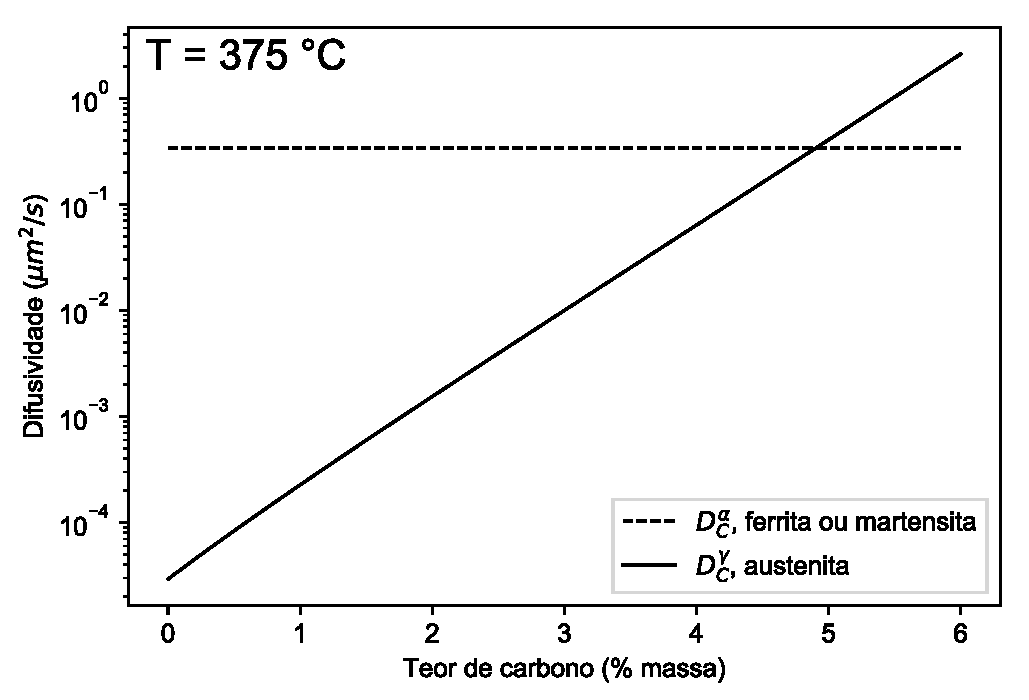
\includegraphics[width=.8\textwidth]{img/difusividades_carbono.pdf}
  \caption{Efeito do teor de carbono nas difusividades de carbono na ferrita (eq. \ref{eq:Agren_ferrita}) e a na austenita (eq. \ref{eq:Agren_austenita}) a \SI{375}{\degreeCelsius}.}
  \label{fig:difusividades}
\end{figure}

O algoritmo de diferenças finitas foi aplicado independentemente em diferentes malhas correspondentes às diferentes fases consideradas no problema. De forma a acoplar todas as malhas sem violar as equações de conservação, as condições de contorno nas interfaces foram definidas de acordo com a equação:

\begin{equation}
  -D_C^\alpha \frac{d c^\alpha}{d z}\Bigg|_{int} + v\left(c^\gamma_{int} - c^\alpha_{int} \right) = -D_C^\gamma \frac{d c^\gamma}{d z}\Bigg|_{int} \label{eq:continuity_int}
\end{equation}

Na interface imóvel martensita/austenita, a equação \ref{eq:continuity_int} avaliada para velocidade $v = 0$ implica que o fluxo de carbono deve ser igual em ambas as fases. Por sua vez, a condição de contorno na interface móvel ferrita bainítica/austenita representa o problema de Stefan, %CITATION NEEDED
em que a velocidade interfacial é determinada pela equação \ref{eq:int_velocity}. A condição de Neumann, representando fluxo zero de carbono, é aplicada nas extremidades dos domínios de cálculo de modo a definir o domínio de simulação como um sistema fechado.

\subsection{Condições de simulação}

A microestrutura inicial das simulações corresponde à obtida no tempo zero da etapa de partição. Assim, assume-se que a microestrutura inicial consiste de uma mistura martensita e austenita com composições idênticas equivalentes à composição da austentita determinada pelos cálculos termodinâmicos (i.e., Fe--0.76C--2.54Si--0.21Mn--0.39Cu); nódulos de grafita não foram considerados. Como discutido anteriormente, as placas de martensita apresentam uma grande dispersão de tamanhos. Placas formadas em temperaturas mais elevadas são mais grosseiras, enquanto placas formadas sob super-resfriamentos maiores são mais refinadas. Dessa forma, de modo a escolher a largura da placa de martensita para as simulações, a largura das maiores placas de martensita foi estimada a partir das microestruturas caracterizadas. Verificou-se que o valor de \SI{1}{\mu m} trata-se de uma boa aproximação para a largura das placas de martensita.

De maneira a reproduzir as condições experimentais, foi escolhida uma fração inicial de martensita compatível com a temperatura de têmpera de \SI{170}{\degreeCelsius}, isto é de 43\%. Sob essa condição a largura do grão não-transformado de austenita é de \SI{1,32}{\mu m}. As simulações foram realizadas assumindo que a etapa de partição é conduzida a \SI{375}{\degreeCelsius} por até 100~s. Para a avaliar o efeito da reação bainítica e a precipitação de carbonetos no interior da martensita, quatro diferentes cenários (representados na Figura \ref{fig:esquema_simulacoes}) foram analisados:

\begin{enumerate}[(a)]
  \item Reação bainítica não acontece e não há precipitação de carbonetos na martensita
  \item Reação bainítica não acontece e há precipitação de carbonetos na martensita
  \item Reação bainítica acontece e não há precipitação de carbonetos na martensita
  \item Reação bainítica acontece e há precipitação de carbonetos na martensita
\end{enumerate}

Nos cenários que levam em conta a reação bainítica é assumido que não há tempo de incubação para a nucleação de ferrita bainítica. Três núcleos de ferrita bainítica são posicionados equiespaçadamente no grão de austenita não transformado, como mostram as figuras \ref{fig:esquema_simulacoes}c e \ref{fig:esquema_simulacoes}d.

\begin{figure}
  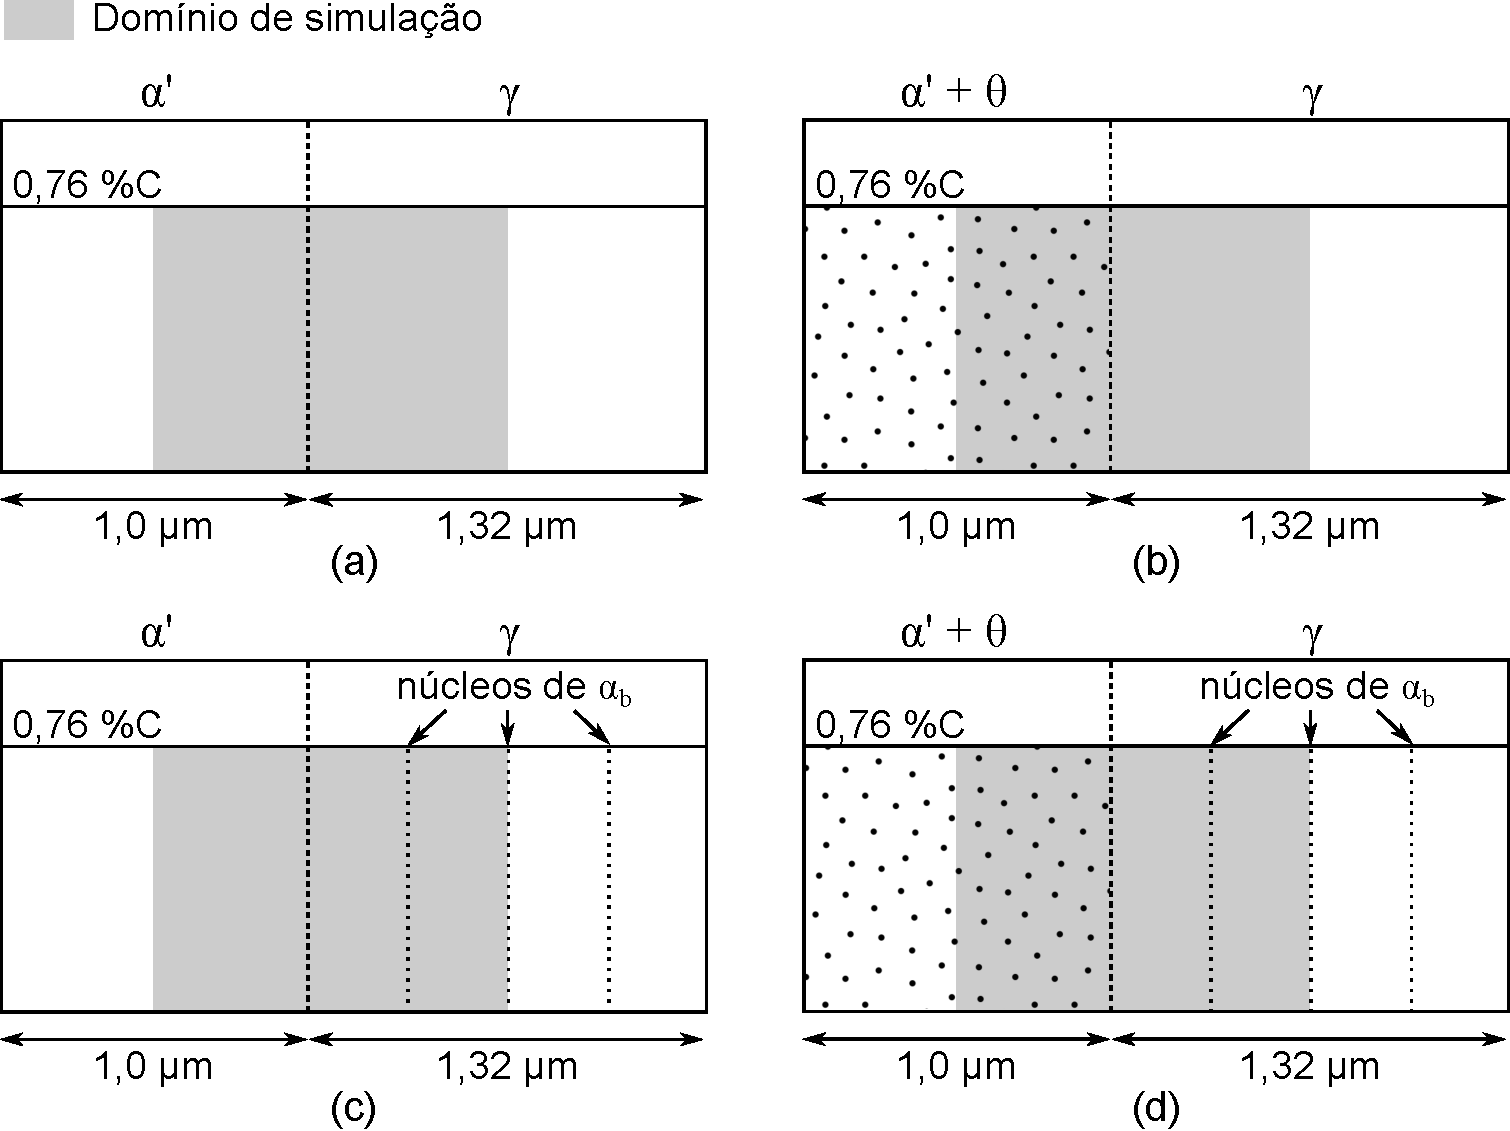
\includegraphics[width=.9\textwidth]{img/cpartition/scheme_simulations.pdf}
  \caption{Desenho esquemático ilustrando os quatro diferentes cenários de simulação considerados: (a) Reação bainítica não acontece e não há precipitação de carbonetos na martensita; (b) Reação bainítica não acontece e há precipitação de carbonetos na martensita; (c) Reação bainítica acontece e não há precipitação de carbonetos na martensita; (d) Reação bainítica acontece e há precipitação de carbonetos na martensita.}
  \label{fig:esquema_simulacoes}
\end{figure}

Os potenciais químicos de C, Si, Mn, Cu e Fe na ferrita e na austenita foram determinados por cálculos termodinâmicos utilizando o banco de dados TCFE8 no software Thermo-Calc\textregistered{} assumindo que a fração de sítios de todas espécies ($y_j$), exceto a do carbono, são iguais aos respectivos valores médios de $y_j$ a \SI{880}{\degreeCelsius} na austenita. Esta consideração está relacionada à hipótese de paraequilíbrio, assumida nas simulações. Isto é, seja durante a partição de carbono, seja no crescimento da ferrita bainítica, apenas a difusão de carbono é considerada, enquanto a redistribuição a longo alcance dos elementos substitucionais é despreza. Esta consideração é razoável para a temperatura de simulação de $\SI{375}{\degreeCelsius}$, pois nesta temperatura a difusão de substitucionais é lenta, e vai de acordo com observações na literatura por tomografia de sonda atômica. % CITATION NEEDED
Vale notar que a lei de Fick como apresentada neste trabalho não seria válida para o problema de difusão multicomponente, que requeria uma formulação do problema baseada nos gradientes de potenciais químicos.

De forma a contabilizar a discrepância entre os limites termodinâmicos previstos computacionalmente e o teor de carbono observado experimentalmente na austenita, os potenciais químicos da ferrita bainítica foram modificados considerando a teoria WBs. De acordo com a extrapolação proposta por Hillert, a energia extra para a reação bainítica a \SI{375}{\degreeCelsius} é de \SI{1787.6}{J/mol}. Esta energia foi somada aos potenciais químicos da ferrita bainítica. O equilíbrio metaestável entre ferrita e austenita calculado utilizando os potenciais químicos modificados resultam no teor de carbono de 1,59\% na austenita. 

\subsection{Influência da precipitação de carbonetos na redistribuição de carbono}

\label{sec:cpartition_sem_bainita}

Na Figura \ref{fig:cprofiles_sem_reacoes} são mostrados os perfis de carbono relativos ao caso em que a redistribuição de carbono entre martensita e austenita acontece sem qualquer reação competitiva. Nota-se que para tempos curtos o teor de carbono na austenita na interface ($c^\gamma_{int}$) estabelece valores altos, muito superiores à composição inicial da liga ($c_0$). O valor máximo de $c^\gamma_{int}$ observado é de $\approx$~4,15\%. Por outro lado, a composição interfacial na martensita ($c^{\alpha'}_{int}$) rapidamente cai para valores próximos de zero. Modelos cinéticos de partição de carbono reportados na literatura, semelhantes a esse, também apresentam esse comportamento\cite{Santofimia2008,Santofimia2009}. O modelo de Santofimia, no entanto, ao contrário do presente modelo, não assume o efeito da composição química na difusividade de carbono da austenita e, em decorrência, os valores observados de $c^\gamma_{int}$ são ainda maiores (> 6\%). Esse comportamento é explicado pela condições de contorno na interface. Partindo da consideração de que os fluxos de carbono na interface são iguais na austenita e na ferrita, necessária para que haja conservação das espécies, e, conquanto não haja ocorrência de \enfase{soft impingement}
na austenita ou martensita, é possível provar que a seguinte relação deve ser obedecida:

\begin{equation}
  \frac{{D_C^{\alpha\text{'}}}_{int}}{{D_C^\gamma}_{int}} = \left(\frac{c^\gamma_{int} - c_0}{c_0 - c^{\alpha'}_{int}}\right)^2
  \label{eq:conservacao_interface}
\end{equation}

\begin{figure}
  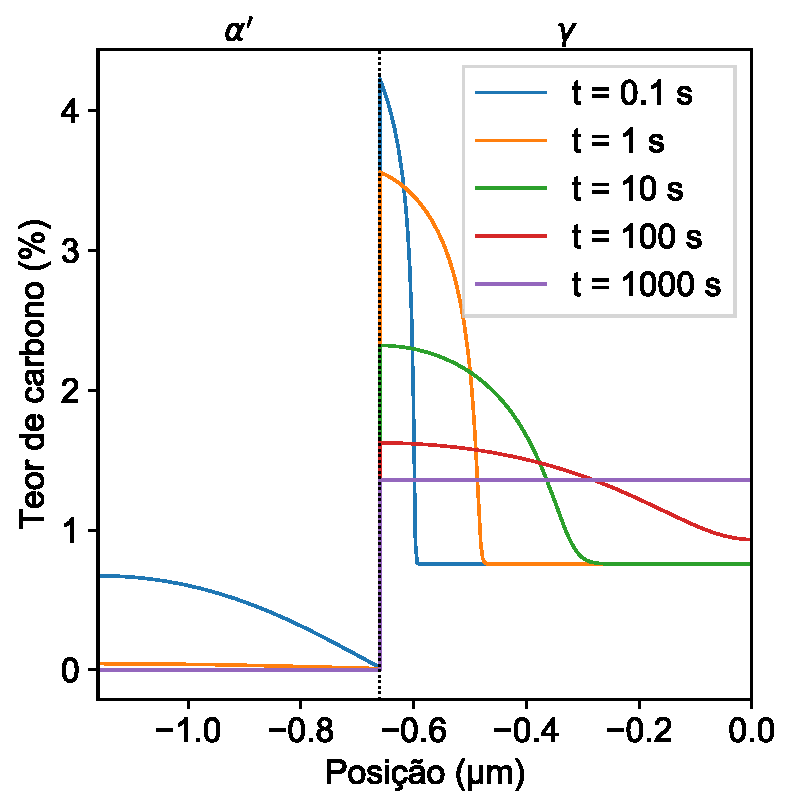
\includegraphics[width=.6\textwidth]{img/cpartition/cprofiles/mart_FoFo_CCE.pdf}
  \caption{Perfis de carbono para o caso em que a partição de carbono entre martensita e austenita calculada sem a consideração de qualquer reação competitiva.}
  \label{fig:cprofiles_sem_reacoes}
\end{figure}

Como mencionado anteriormente, a difusividade de carbono na austenita aumenta exponencialmente com o aumento do teor de carbono. Assim, a alta concentração de carbono na interface leva a um aumento local da difusividade de carbono, diminuindo a razão $\frac{{D_C^{\alpha\text{'}}}_{int}}{{D_C^\gamma}_{int}}$. Assim, quando o efeito da dependência de $D^\gamma_C$ é considerado, $c^\gamma_{int}$ e $c^{\alpha'}_{int}$ devem ser menores para que a equação \ref{eq:conservacao_interface} seja satisfeita. Para um tempo suficientemente longo ocorre o \enfase{soft impingement} dos perfis de difusão na martensita, fazendo com que as composições interfaciais diminuam. Isso ocorre para aproximadamente $t > \SI{0,1}{s}$. Vale salientar que $c^\gamma_{int}$ e $c^{\alpha'}_{int}$ dependem um do outro pelo equilíbrio local de carbono (igualdade dos potenciais químicos de carbono) e, portanto, não podem ser arbitrariamente alterados.

O fato de $c^{\alpha'}_{int}$ decrescer a zero para tempos curtos implica que a difusão de carbono da martensita para a austenita ocorre rapidamente, sendo controlada pela difusão de carbono na martensita. Isso pode ser melhor observado na Figura \ref{fig:cavg_sem_reacoes}, que mostra a evolução das composições médias da martensita e da austenita. 99\% de todo o carbono antes presente na martensita é particionado para a austenita em apenas 2,2~s. Por outro lado, como a difusão na austenita é mais lenta do que na martensita, o carbono particionado para a austenita demora consideravelmente mais para se homogeneizar ao longo de todo o grão. Um perfil de carbono ``plano'' na austenita, que denota esta homogeneização, é obtido apenas para $t > \SI{500}{s}$

\begin{figure}
  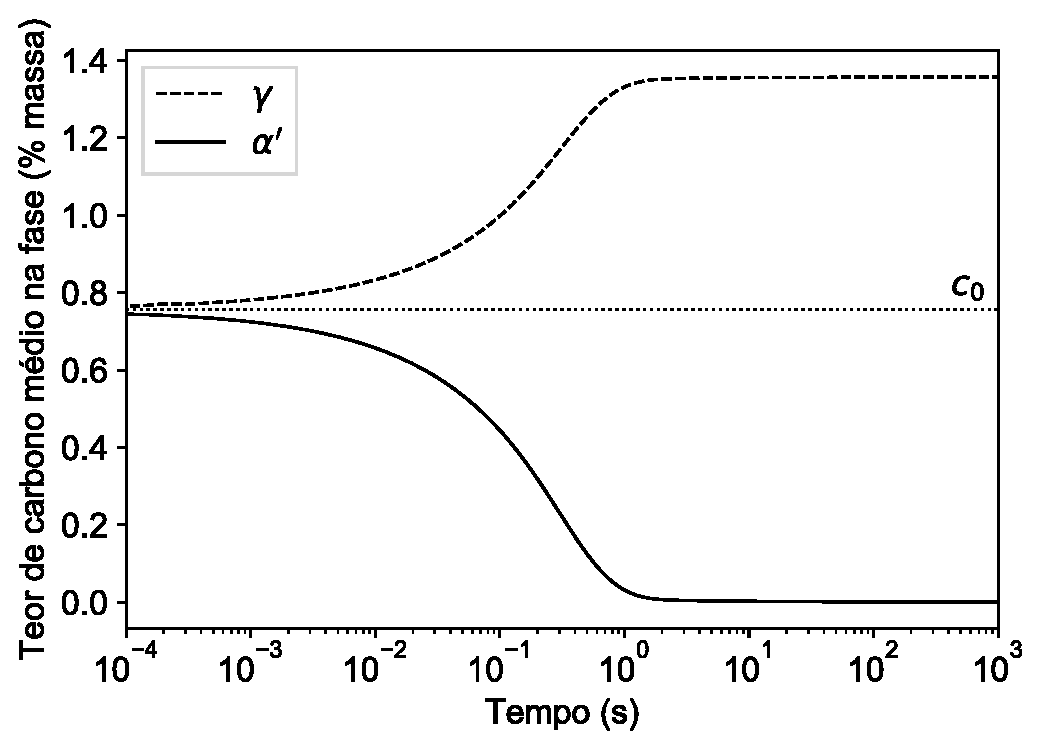
\includegraphics[width=.8\textwidth]{img/cpartition/CCE_cavg.pdf}
  \caption{Evolução do teor de carbono médio na martensita $\alpha'$ e na austenita $\gamma$ calculada para a condição em que reações competitivas não são consideradas.}
  \label{fig:cavg_sem_reacoes}
\end{figure}

No modelo modificado que considera a precipitação de carbonetos na martensita, assume-se que os carbonetos já estão precipitados na martensita no instante $t = 0$ da etapa de partição, já havendo estabelecido o equilíbrio metaestável $\alpha' + \theta$.
A evidência experimental de carbonetos na martensita para tempos muito curtos justifica esse pressuposto.
A mistura $\alpha' + \theta$ foi assumida como uma única pseudofase cuja difusividade é calculada ponderando a difusividade da martensita pela sua fração de fase, ou seja, descontando a fração de carbonetos. A fração de carbonetos, por sua vez, é calculada por meio da aplicação da regra das alavancas assumindo 
% que a estequiometria do carboneto é $M_3C$ (25\% atômico de C) e 
que o teor de carbono da martensita é equivalente ao limite de solubilidade da ferrita na temperatura de partição (0,012\% a \SI{375}{\degreeCelsius}). 

Uma vez que o modelo ERC$\theta$ prevê diferentes composições de carbono dependendo da energia livre dos carbonetos, é esperado que isto afetará a cinética de redistribuição de carbono. Assim, cenários considerando carbonetos com diferentes energias livres foram avaliados nas simulações. Os parâmetros termodinâmicos relativos à pseudofase $\alpha' + \theta$ para as diferentes condições de simulação consideradas nesta seção são mostradas na Tabela \ref{tab:cpartition_CCEtheta}. Os casos abordados abrangem a precipitação de orto e paracementita e casos intermediários em que foram definidos carbonetos com valores de potencial químico de carbono $\mu_C$ intermediários aos da orto e paracementita. $\mu_C$ é diretamente relacionado à energia livre do carboneto $G$ pela relação termodinâmica:

\begin{equation}
  G = \sum x_j \mu_j
\end{equation} 
%
em que $x_j$ é a fração molar do elemento $j$ no carboneto. Fica evidente que quanto maior $\mu_C$, maior é $G$ (i.e., \enfase{menos estável} é o carboneto), ainda que $G$ dependa da estequiometria do carboneto considerado; por exemplo, para a orto e paracementita (ambos do tipo $Fe_3C$), $x_C = \SI{0.25}{}$. Por outro lado, carbonetos de transição usualmente são mais ricos em carbono do que a cementita, apresentando $x_C \approx \SI{0.3}{}$ (e.g., para o carboneto $\epsilon$, $Fe_{2,2}C$, $x_C \approx \SI{0.31}{}$). Ou seja, nesses carbonetos $\mu_C$ possui um peso maior no cálculo de $G$. De toda a forma, a única informação necessária para determinação das condições de contorno nas simulações é a composição interfacial na austenita $c^\gamma_{int}$, calculada pelo modelo ERC$\theta$. Para o cálculo de $c^\gamma_{int}$ é necessário apenas o valor de $\mu_C$ e, assim, a determinação do valor correto de $G$ é um procedimento redundante.
% Devido à evidência experimental de carbonetos de transição durante no ferro fundido T\&P particionado a \SI{375}{\degreeCelsius}, $G$ foi estimado assumindo $x_C = \SI{0.30}{}$ e que os carbonetos se formam sem partição de solutos substitucionais com a martensita (ou seja, também são parafases).

\begin{table}
  \centering
  \caption{Parâmetros termodinâmicos utilizados para as simulações da partição de carbono entre $\alpha' + \theta$ e $\gamma$.}
  \begin{tabular}{cccc}
    \hline
    Condição & $\mu_C$ (kJ/mol) & $c^\gamma_{int}$ (\% massa) & Valor relativo de $c^\gamma_{int}$\\
    \hline
    Ortocementita (Fig. \ref{fig:cprofiles_sem_bainita}a) & 8,189 & 0,227 & $c^\gamma_{int} < c_0 < ERC$ \\
    & 16,434 & 0,757 & $c^\gamma_{int} = c_0 < ERC$ \\
    (Fig. \ref{fig:cprofiles_sem_bainita}c) & 20,000 & 1,151 & $c_0 < c^\gamma_{int} < ERC$ \\
    & 23,207 & 1,590 & $c_0 < ERC < c^\gamma_{int}$ \\
    & 25,000 & 1,866 & $c_0 < ERC < c^\gamma_{int}$ \\
    & 30,000 & 2,729 & $c_0 < ERC < c^\gamma_{int}$ \\
    Paracementita (Fig. \ref{fig:cprofiles_sem_bainita}b) & 35,511 & 3,795 & $c_0 < ERC < c^\gamma_{int}$ \\
    \hline
  \end{tabular}
  \label{tab:cpartition_CCEtheta}
\end{table}

Na Figura \ref{fig:cprofiles_sem_bainita}a são mostrados os perfis de carbono obtidos assumindo que o carboneto precipitado é a ortocementita. A precipitação de ortocementita leva a uma composição interfacial na austenita ($c^\gamma_{int} = \SI{0.17}{\%}$) inferior ao carbono inicial (0,76\%). Assim, nessa condição a difusão de carbono ocorre da austenita para a martensita e o aumento de carbono em $\alpha' + \theta$ é refletido no aumento da fração de carbonetos.

\begin{figure}
  \subfloat[ortocementita]{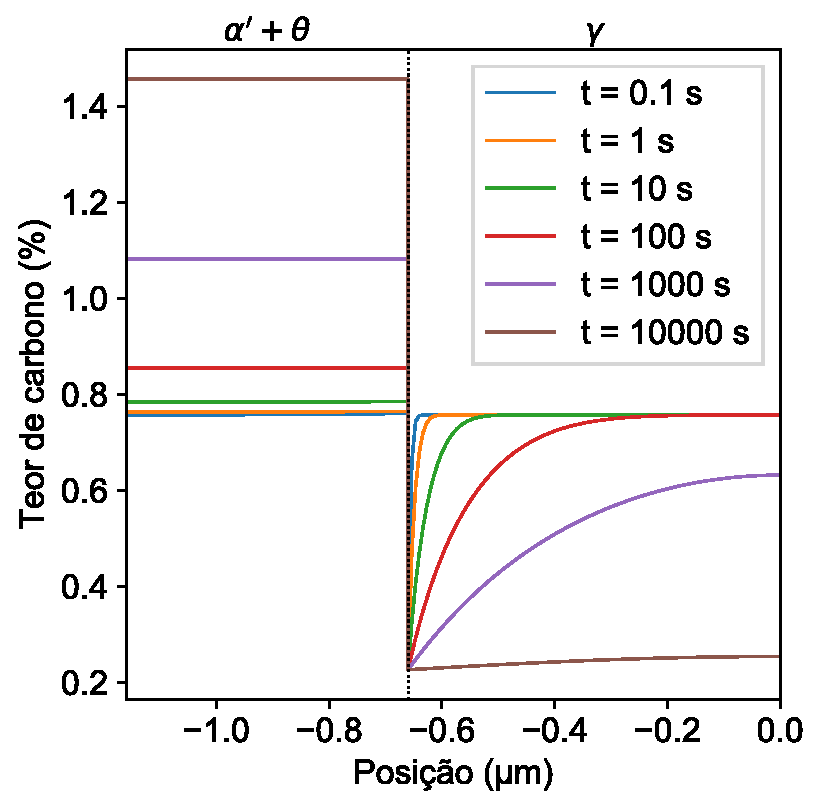
\includegraphics[width=.48\textwidth]{img/cpartition/cprofiles/mart_FoFo_CCEortho.pdf}}\quad
  \subfloat[paracementita]{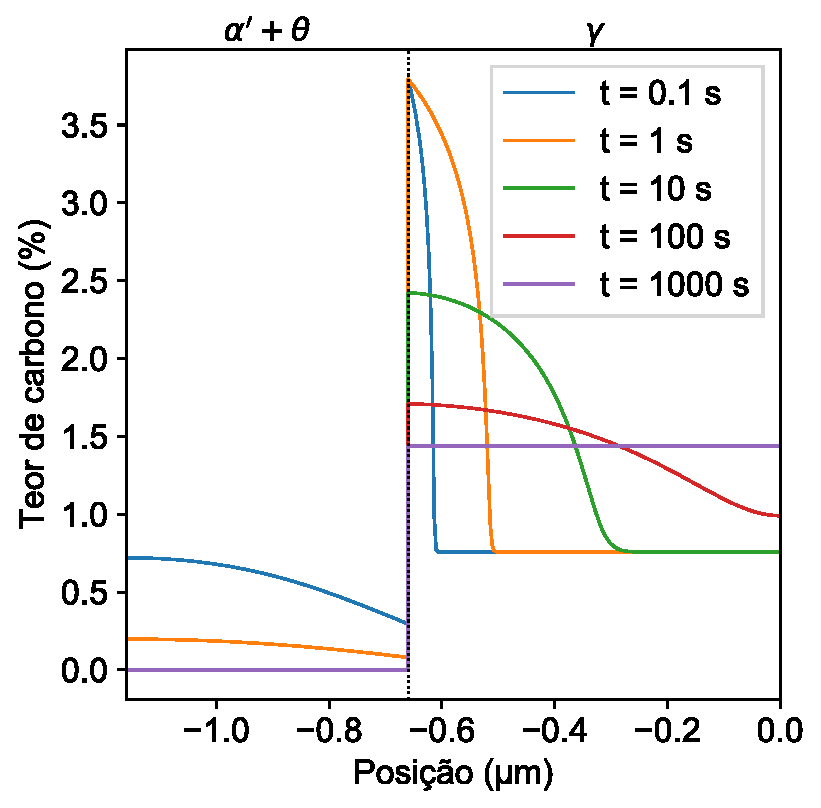
\includegraphics[width=.48\textwidth]{img/cpartition/cprofiles/mart_FoFo_CCEpara.pdf}}\\
  \subfloat[$\mu_C = \SI{20}{kJ/mol}$]{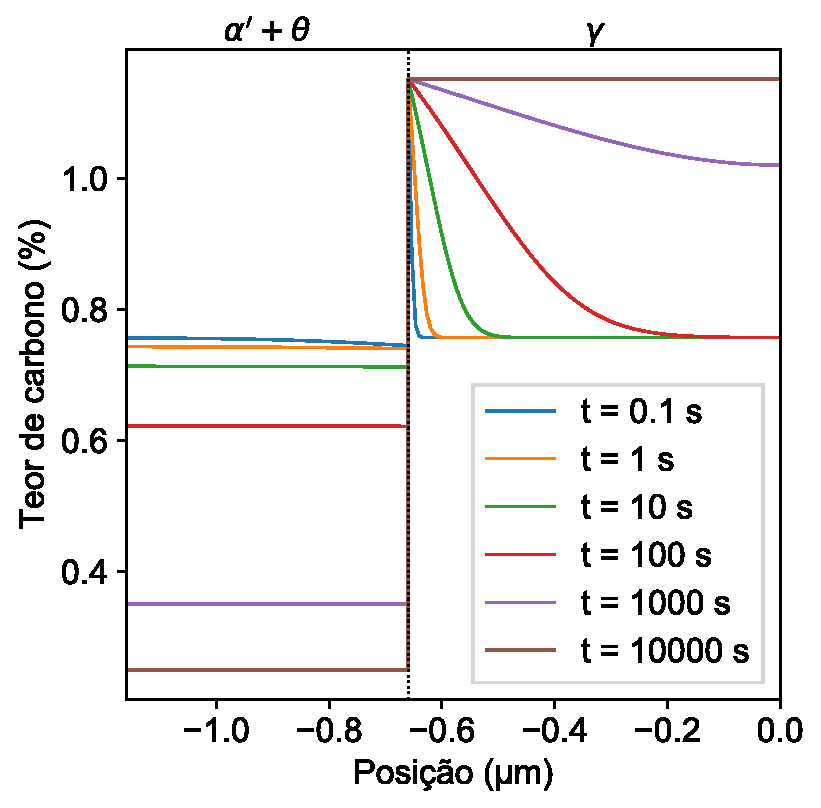
\includegraphics[width=.48\textwidth]{img/cpartition/cprofiles/mart_FoFo_mu20e3.pdf}}
  \caption{Perfis de carbono calculados considerando a presença de carbonetos precipitados na martensita (pseudofase $\alpha' + \theta$).}
  \label{fig:cprofiles_sem_bainita}
\end{figure}

A Figura \ref{fig:cprofiles_sem_bainita}b mostra os perfis de carbono para a situação em que os carbonetos precipitados são de paracementita. Para tempos curtos, $c^\gamma_{int}$ é determinado pelo modelo ERC$\theta$, sendo equivalente a 3,82\%, maior do que a composição inicial. Assim, ao contrário do caso anterior, a partição de carbono de $\alpha' + \theta$ para $\gamma$ de fato ocorre. Devido ao efeito do carbono na difusividade da austenita, o alto carbono na interface se reflete em uma difusão de carbono rápida e a partição de carbono de $\alpha' + \theta$ para $\gamma$ também ocorre rapidamente. Uma vez que o carbono na austenita decresce para valores inferiores à solubilidade de carbono na ferrita (0,012\%) a fração de carbonetos atinge zero. Assim, na ausência de carbonetos as composições interfaciais deixam de ser determinadas pela condição ERC$\theta$ e passam a ser ditadas pela condição ERC, como na primeira simulação. Essa situação é observada, por exemplo, a $t=\SI{10}{s}$.

Os perfis de carbono relativos ao caso em que $\mu_C = \SI{20}{kJ/mol}$ são mostrados na Figura \ref{fig:cprofiles_sem_bainita}c. Como pode ser observado na Tabela \ref{tab:cpartition_CCEtheta}, tanto o valor de $\mu_C = \SI{20}{kJ/mol}$ quanto a composição interfacial na austenita calculada pelo modelo ERC$\theta$ ($c^\gamma_{int} = \SI{1.15}{\%}$) correspondem a valores intermediários aos obtidos para orto e paracementita. $c^\gamma_{int}$ é maior do que a composição inicial, logo a partição de carbono para a austenita ocorre. No entanto, ao contrário do que acontece na presença de paracementita, o carbono em $\alpha' + \theta$ não decresce a zero. Isto acontece em decorrência do fato de que $c^\gamma_{int}$ calculado pelo modelo $ERC\theta$ é inferior à composição calculada pelo modelo ERC a \SI{170}{\degreeCelsius} (1,355\%). Nessas condições, o carbono em $\gamma$ se homogeniza antes de que todo o carbono em $\alpha' + \theta$ seja particionado. 
% novamente devido ao efeito da composição na difusividade, a difusão de carbono na interface é mais lenta do que quando há a precipitação de paracementita. 
% DISCUTIR TEMPO PARA HOMOGENEIZAÇÃO DO CARBONO NA AUSTENITA

O efeito da energia livre dos carbonetos na cinética de redistribuição de carbono é mostrado na Figura \ref{fig:nobainite_cavg}, na qual são apresentadas as curvas da evolução do teor médio de carbono em $\alpha' + \theta$ ($\overline{c^{\alpha' + \theta}}$) com o tempo de partição. Fica evidente que na presença de carbonetos com maiores valores de $\mu_C$ --- isto é, carbonetos menos estáveis, com maior energia livre --- a partição de carbono da martensita para a austenita é acelerada. Quanto maior $\mu_C$, o comportamento da curva de $\overline{c^{\alpha' + \theta}}$ mais se aproxima da condição em que a precipitação de carbonetos é suprimida.
Como discutido anteriormente, um maior $\mu_C$ implica em uma composição $c^\gamma_{int}$ mais elevada, levando à uma difusão de carbono mais rápida na interface.
Por outro lado, caso os carbonetos sejam muito estáveis, causando $c^\gamma_{int} < c_0$, a difusão de carbono acontece de $\alpha' + \theta$ para $\gamma$.

\begin{figure}
  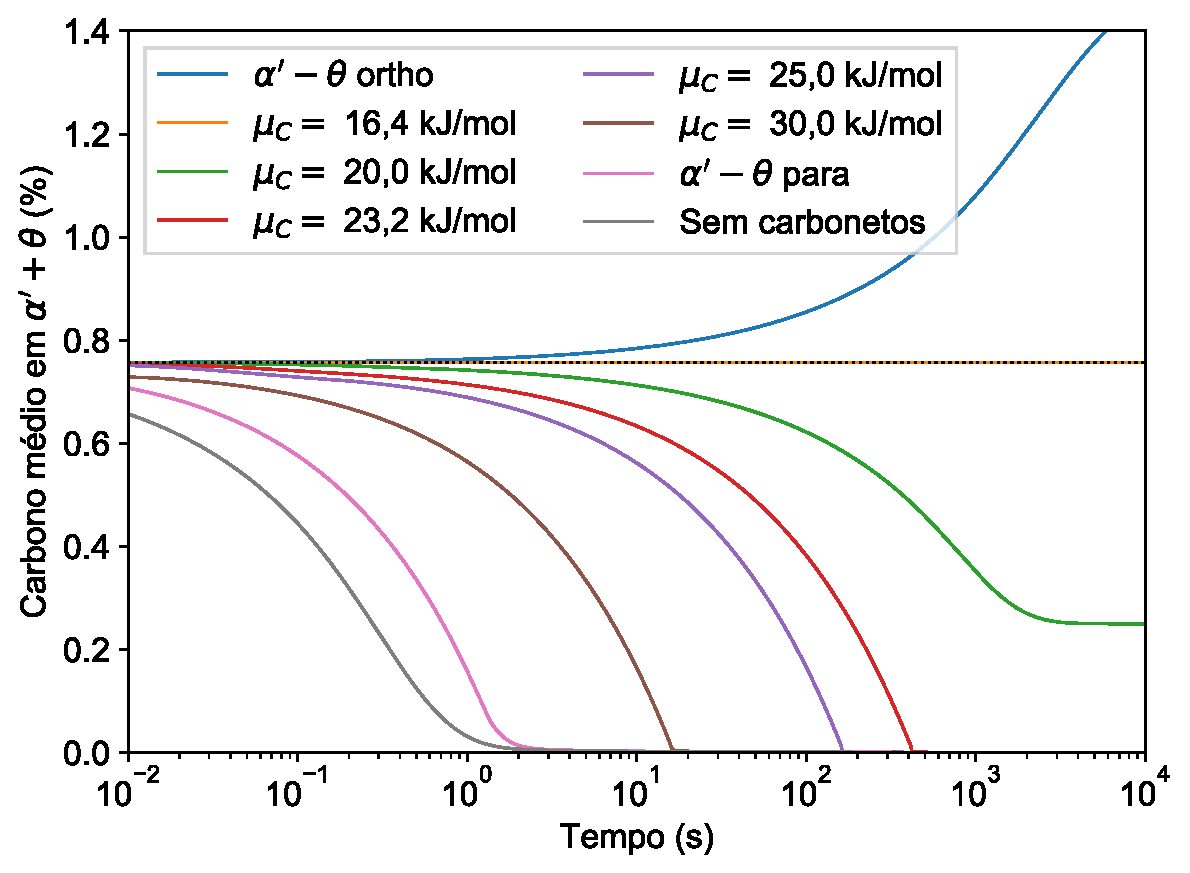
\includegraphics[height=.6\textwidth]{img/cpartition/nobainite_cavg.pdf}
  \caption{Evolução do teor de carbono médio na pseudofase $\alpha' + \theta$ ($\overline{c^{\alpha' + \theta}}$) com o tempo de partição calculada para cenários considerando carbonetos com diferentes energias livres.}
  \label{fig:nobainite_cavg}
\end{figure}

Vale notar que para um valor crítico de $\mu_C = \SI{16.434}{kJ/mol}$, que causa $c^\gamma_{int} = c_0$, não há formação de um gradiente de carbono na austenita e, portanto, não há redistribuição de carbono entre $\alpha' + \theta$ e $\gamma$.

Para $\mu_C = \SI{20}{kJ/mol}$ a partição de carbono não é completa e $\overline{c^{\alpha' + \theta}}$ estabelece um patamar ao final da etapa de partição. Isto acontece porque $c^\gamma_{int}$ assume um valor maior do que $c_0$, mas menor do que a composição da austenita calculada pelo modelo ERC de Speer. 
É importante ressaltar que a composição ERC da austenita é dependente da fração inicial de martensita, sendo para a temperatura de têmpera de \SI{170}{\degreeCelsius} igual a 1,355\%. O valor de $\mu_C$ correspondente à composição $c^\gamma_{int} = \SI{1.355}{\%}$ é de $\SI{21.556}{kJ/mol}$. Dessa forma, em sistemas com carbonetos com $\mu_C$ inferiores a $\SI{21.556}{kJ/mol}$ a partição de carbono não é completa. Apenas se $\mu_C$ for superior a $\SI{21.556}{kJ/mol}$ a partição será completa.

% Isso acontece porque há também um valor crítico de $\mu_C$ para o qual $c^\gamma_{int} = ERC$. Para carbonetos que levam a valores inferiores a este $\mu_C$ crítico, $c^\gamma_{int}$ é inferior a ERC e a partição de carbono não é completa. É importante ressaltar que a composição ERC da austenita é dependente da fração inicial de martensita. 
% Dessa forma, o valor de $\mu_C$ crítico depende da temperatura de têmpera. Para a temperatura de têmpera, em que a composição ERC equivale a 1,355\%, $\mu_C$ crítico é igual $\mu_C = \SI{21.556}{kJ/mol}$.

\subsection{Influência da reação bainítica na redistribuição de carbono}

Os perfis de carbono para a condição de simulação que assume que há reação bainítica, mas não há precipitação de carbonetos na martensita, são mostrados na Figura \ref{fig:cprofiles_sem_carbonetos_sep}. Na figura os perfis de carbono originais da simulação foram refletidos ao longo da coordenada $z = 0$ (isso é somente possível devido à condição de contorno de Neumann aplicada nesta posição), de modo a representar a nucleação das três placas de ferrita bainítica na extensão total do grão original não-transformado de austenita. De modo a facilitar a explicação dos resultados, as diferentes regiões são nomeadas da seguinte forma:

\begin{itemize}
  \item $\alpha_{b1}$: placas de ferrita bainítica nucleadas a $z = \SI{-0.33}{\mu m}$ e $z = \SI{0.33}{\mu m}$ (as duas são equivalentes devido à condição de simetria em $z = 0$);
  \item $\alpha_{b2}$: placa de ferrita bainítica nucleada a $z = 0$;
  \item $\gamma_1$: blocos de austenita adjacentes à martensita e a $\alpha_{b1}$;
  \item $\gamma_2$: bloco de austenita entre as placas de ferrita bainítica $\alpha_{b1}$ e $\alpha_{b2}$;
  \item $int_1$: interfaces entre $\alpha_{b1}$ e $\gamma_1$;
  \item $int_2$: interfaces entre $\alpha_{b1}$ e $\gamma_2$;
  \item $int_3$: interfaces entre $\alpha_{b2}$ e $\gamma_2$.
\end{itemize}

\begin{figure}
  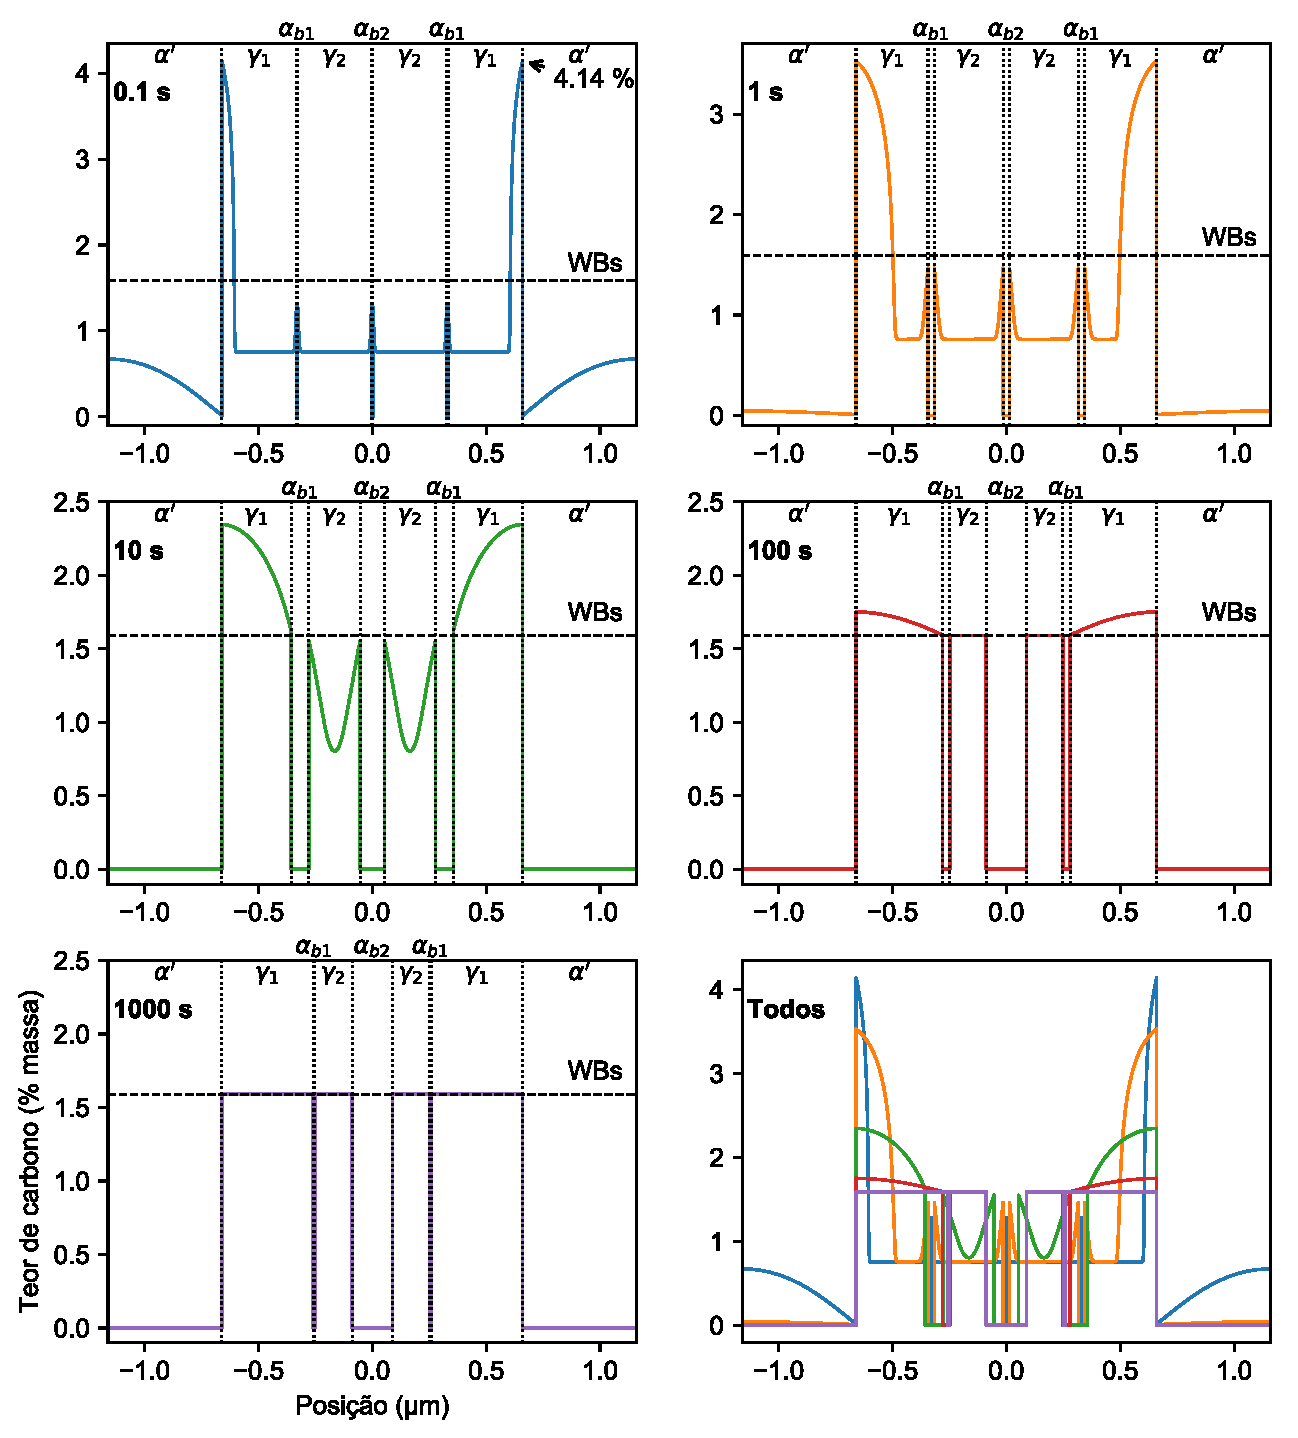
\includegraphics[width=\textwidth]{img/cpartition/cprofiles/coupled_FoFo_375_CCE_sep.pdf}
  \caption{Perfis de carbono calculados para o caso em que não há precipitação de carbonetos na martensita e ocorre reação bainítica na austenita.}
  \label{fig:cprofiles_sem_carbonetos_sep}
\end{figure}

% As linhas verticais representam a posição das interfaces ao final da simulação.
Como na situação em que a reação bainítica não é considerada, para tempos curtos os perfis de carbono na austenita são acentuados nas proximidades da interface martensita/austenita e se atenuam para tempos crescentes. A composição interfacial da martensita descresce rapidamente para valores próximos de zero, levando a um processo de partição de carbono controlado pela difusão na martensita. Por sua vez, a redistribuição de carbono nas proximidades das placas de $\alpha_b$ é melhor analisada utilizando Figura \ref{fig:cprofiles_sem_carbonetos_tracking}, que mostra em detalhe estas regiões. As linhas pontilhadas representam os lugares geométrico dos pares ordenados posição--teor de carbono da austenita na interface ($c^\gamma_{int}$). 

\begin{figure}
  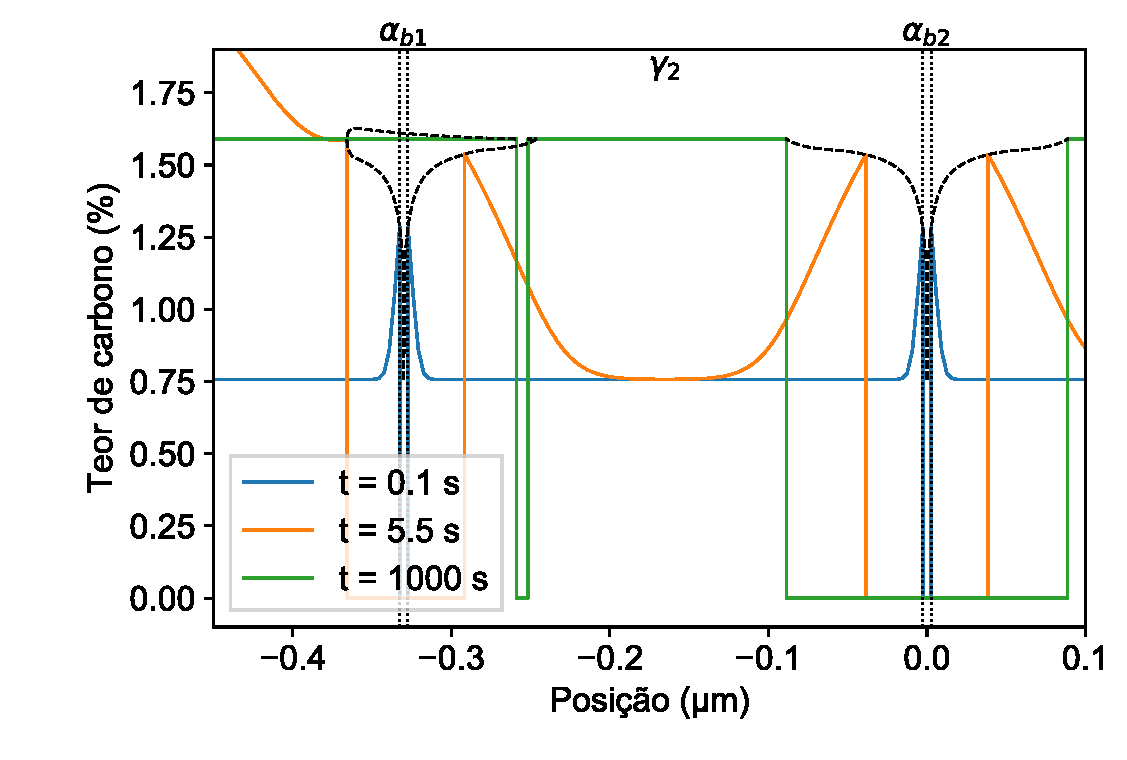
\includegraphics[width=.8\textwidth]{img/cpartition/cprofiles/coupled_FoFo_375_CCE_tracking.pdf}
  \caption{Detalhe da Figura \ref{fig:cprofiles_sem_carbonetos_sep} mostrando a evolução das posições das interfaces entre as placas de ferrita bainítica e a austenita. Nota-se que a placa $\alpha_{b1}$ inicialmente cresce, mas se redissolve para tempos longos de partição.}
  \label{fig:cprofiles_sem_carbonetos_tracking}
\end{figure}

Observa-se que as composições interfaciais $c^\gamma_{int}$ aumentam conforme as interfaces avançam. Isso decorre da natureza do modelo de modo misto. Ao contrário da suposição de equilíbrio local de Zener, em que as composições interfaciais são definidas pelo equilíbrio termodinâmico, no modelo de modo misto é assumido o equilíbrio local de carbono (isto é, $\mu_C^\gamma = \mu_C^{\alpha_b}$). De fato, a força motriz para o avanço da interface se origina das diferenças de potenciais químicos do ferro e dos elementos substitucionais, isto é, a força motriz é surge a partir da própria situação de não-equilíbrio na interface. Conforme a interface avança e carbono é rejeitado para a austenita, o teor de carbono aumenta gradativamente até atingir o equilíbrio termodinâmico e a interface para. Nas considerações do presente modelo o teor de carbono no equilíbrio é a composição WBs.

Nota-se que o comportamento da movimentação da interface é diferente dependendo da interface analisada. As interfaces $int_2$ e $int_3$ se movimentam de forma semelhante, avançando para o interior do bloco de austenita $\gamma_2$, de acordo com a descrição de acima. Por outro lado, a interface $int_1$ inicialmente avança em direção à austenita $\gamma_1$, mas a aproximadamente $t \approx \SI{5.5}{s}$ o sentido da movimentação da interface se reverte e $\alpha_{b1}$ passa a redissolver. Isto é acompanhado de um rápido aumento da composição interfacial $c^\gamma_{int_1}$. Tal comportamento pode ser também visualizado na Figura \ref{fig:evolucao_interface_bainita}a, que mostra a evolução de $c^\gamma_{int_1}$ e da posição da interface $int_1$ com o tempo. Esse fenômeno pode ser explicado pela rápida partição de todo carbono da martensita para austenita, que acontece para tempos curtos ($\approx \SI{1}{s}$). O carbono acumulado na austenita faz com que a composição na interface $int_1$ aumente, fazendo que o potencial químico de carbono aumente localmente. Isto faz com que a força motriz para movimentação da interface, que antes era positiva --- favorecendo o crescimento de $\alpha_{b1}$ --- passe a ser negativa (vide Figura \ref{fig:evolucao_interface_bainita}b), e a interface $int_1$ passa a receder. Uma vez que $\alpha_{b1}$ começa a redissolver e, consequentemente, $\gamma_1$ passa a crescer, o carbono se espalha pela austenita e a composição $c^\gamma_{int_1}$ volta a decrescer, até eventualmente atingir a composição WBs de equilíbrio. Nesse caso em específico, após 1000~s a placa de ferrita bainítica $\alpha_{b1}$ não se dissolve por completo. A possibilidade de um placa $\alpha_b$ se dissolver por completo é condicionada à geometria de simulação. Caso a placa de $\alpha_b$ esteja mais próxima da martensita, $\alpha_b$ será mais intensamente afetado pelo fluxo de carbono proveniente da martensita e, neste caso, maior é a possibilidade da placa se dissolver por completo. Tal situação seria observada, por exemplo, quando o material é temperado em temperaturas mais baixas e os blocos de austenita são menores.

\begin{figure}
  \subfloat[]{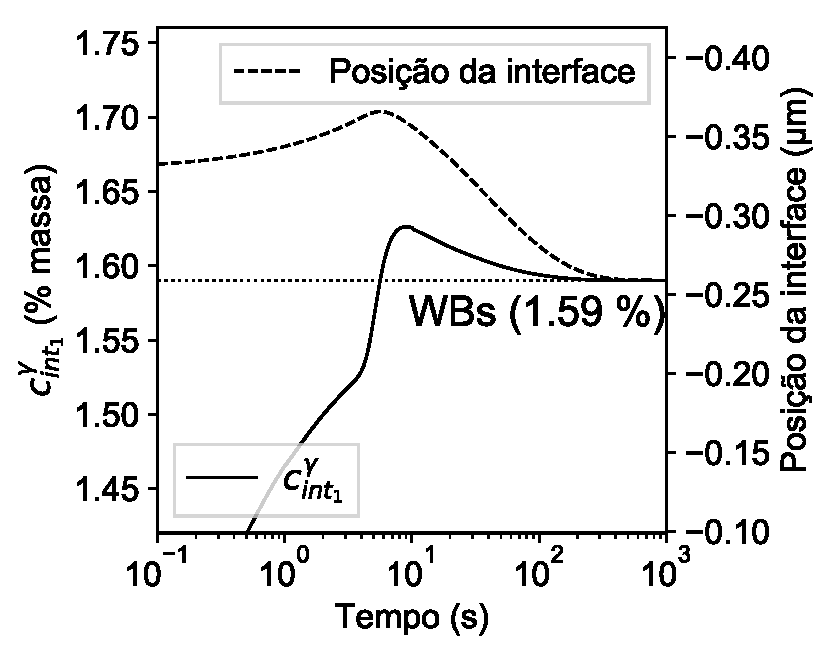
\includegraphics[height=.4\textwidth]{img/cpartition/aus1fer1_interface_comp.pdf}}\quad
  \subfloat[]{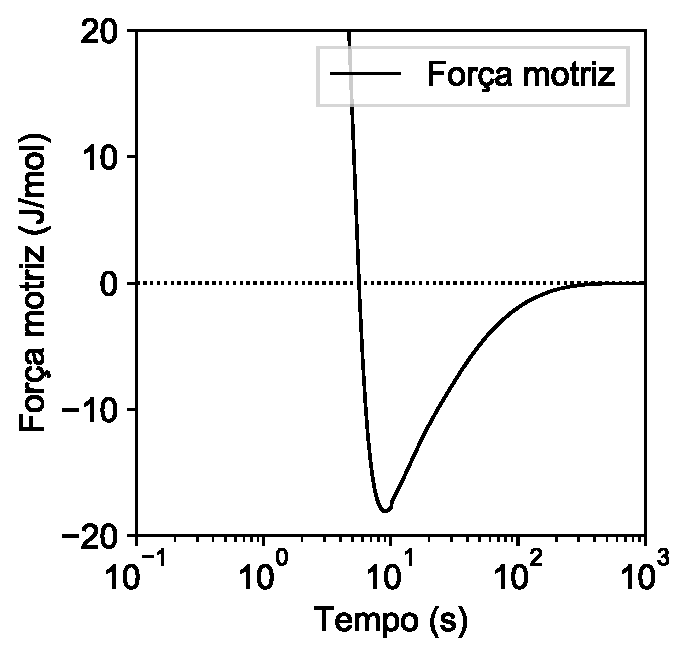
\includegraphics[height=.4\textwidth]{img/cpartition/aus1fer1_interface_DF.pdf}}
  \caption{Evolução de diferentes parâmetros da interface $int_1$ entre $\alpha_{b1}$ e $\gamma_1$. (a) Composição interfacial $c^\gamma_{int_1}$ (linha sólida) e posição da interface (linha tracejada). (b) Força motriz para movimentação da interface.}
  \label{fig:evolucao_interface_bainita}
\end{figure}

A redistribuição de carbono no material também pode ser entendida como um processo de homogeneização do potencial químico de carbono $\mu_C$. De fato, a verdadeira força motriz para difusão se origina de gradientes de energia livre, que, para pressão e temperatura constantes, emerge dos gradientes de potenciais químicos. A Figura \ref{fig:muprofiles_sem_carbonetos} mostra os perfis de $\mu_C$ correspondentes aos perfis de carbono mostrados na Figura \ref{fig:cprofiles_sem_carbonetos_sep}. Percebe-se que os perfis de $\mu_C$ tendem a se homogeneizar para tempos crescentes. Nas interfaces entre austenita e martensita ou ferrita bainítica, $\mu_C$ é um ponto invariante, de acordo com a hipótese de equilíbrio local de carbono assumida nas simulações.

\begin{figure}
  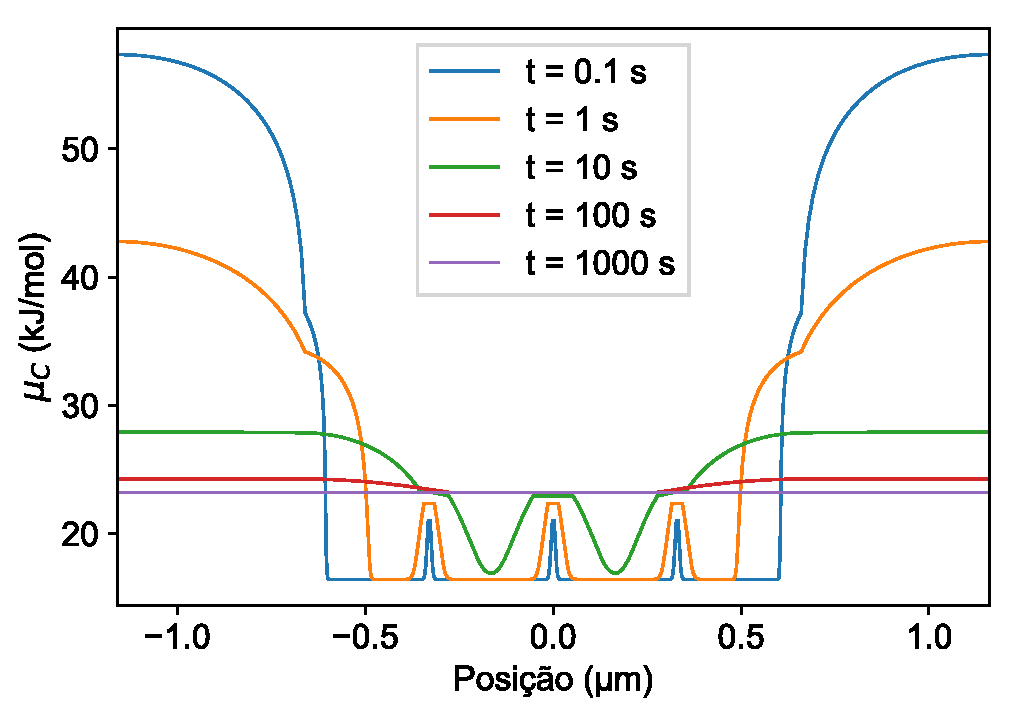
\includegraphics[width=.8\textwidth]{img/cpartition/muprofiles/coupled_FoFo_375_CCE.pdf}
  \caption{Perfis de potencial químico de carbono $\mu_C$ correspondentes aos perfis de carbono mostrados na Figura \ref{fig:cprofiles_sem_carbonetos_sep}, isto é, para o caso em que a reação bainítica é considerada e a precipitação de carbonetos é desprezada.}
  \label{fig:muprofiles_sem_carbonetos}
\end{figure}

\subsection{Interação entre reação bainítica e precipitação de carbonetos}

Os casos mais complexos avaliados pelo presente modelo são aqueles em que tanto a reação bainítica quanto a precipitação de carbonetos na martensita são considerados. Em relação à reação bainítica, a mesma disposição utilizada no exemplo anterior foi usada nos problemas apresentados nesta seção. Em relação à precipitação de carbonetos, foram avaliados carbonetos com diferentes energias livres, tal qual a avaliação apresentada na seção \ref{sec:cpartition_sem_bainita}. As informações termodinâmicas relativas às diferentes condições de simulação são resumidas na Tabela \ref{tab:cpartition_CCEtheta}.

\begin{table}
  \centering
  \caption{Parâmetros termodinâmicos utilizados para as simulações de redistribuição de carbono assumindo tanto a precipitação de carbonetos quanto a reação bainítica.}
  \begin{tabular}{cccc}
    \hline
    Condição & $\mu_C$ (kJ/mol) & $c^\gamma_{int}$ (\% massa) & Valor relativo de $c^\gamma_{int}$\\
    \hline
    Ortocementita (Fig. \ref{fig:cprofiles_coupled_CCEortho}) & 8,189 & 0,227 & $c^\gamma_{int} < c_0 < WBs$ \\
    & 16,434 & 0,757 & $c^\gamma_{int} = c_0 < WBs$ \\
    & 20,000 & 1,151 & $c_0 < c^\gamma_{int} < WBs$ \\
    (Fig. \ref{fig:cprofiles_coupled_mu23e3}) & 23,207 & 1,590 & $c_0 < c^\gamma_{int} = WBs$ \\
    & 25,000 & 1,866 & $c_0 < WBs < c^\gamma_{int}$ \\
    & 30,000 & 2,729 & $c_0 < WBs < c^\gamma_{int}$ \\
    Paracementita (Fig. \ref{fig:cprofiles_coupled_CCEpara}) & 35,511 & 3,795 & $c_0 < WBs < c^\gamma_{int}$ \\
    \hline
  \end{tabular}
  \label{tab:cpartition_bainite_CCEtheta}
\end{table}

Na Figura \ref{fig:cprofiles_coupled_CCEortho} são mostrados os perfis de carbono relativos à simulação em que a precipitação de ortocementita é considerada. Assim como demonstrado na simulação sem presença de bainita, a formação de ortocementita faz com que a composição interfacial $c^\gamma_{int}$ seja menor do que a composição $c_0$. O carbono que é rejeitado pelo crescimento de ferrita bainítica $\alpha_{b1}$ se acumula na austenita $\gamma_1$, criando um gradiente de composição à frente da interface $(\alpha' + \theta)/\gamma_1$, favorecendo a difusão de carbono de $\gamma_1$ para $\alpha' + \theta$. Por outro lado, os blocos de austenita centrais $\gamma_2$, que não estão em contato com a martensita, não são susceptíveis aos efeitos do acúmulo de carbono na austenita proveniente da partição da martensita. Assim, para tempos longos estes blocos de austenita atingem a composição WBs de equilíbrio.

\begin{figure}
  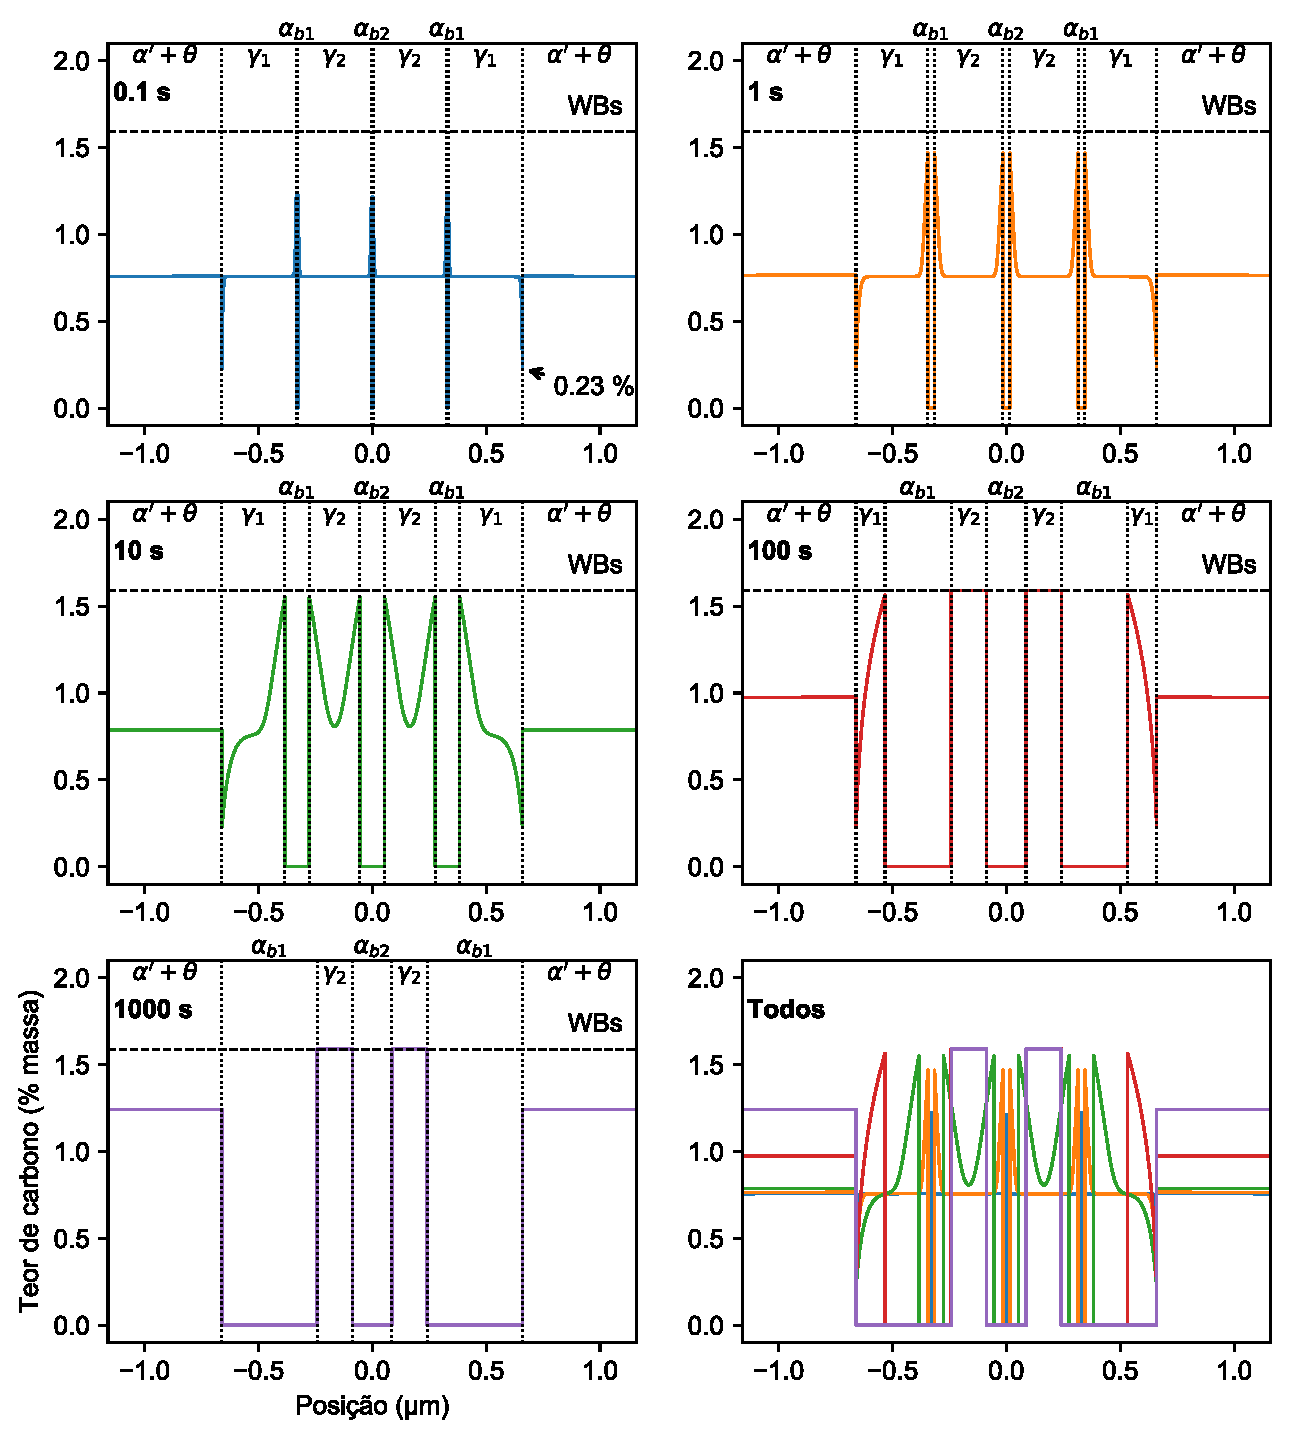
\includegraphics[width=.9\textwidth]{img/cpartition/cprofiles/coupled_FoFo_375_CCEortho_sep.pdf}
  \caption{Perfis de carbono calculados para o caso em que é assumida a precipitação de ortocementita na martensita e ocorre reação bainítica na austenita.}
  \label{fig:cprofiles_coupled_CCEortho}
\end{figure}

O gradiente de carbono em $\gamma_1$ persiste mesmo para tempos longos de partição, já que a composição $c^\gamma_{int}$ é fixada pela condição ERC$\theta$. Consequentemente, devido às leis de conservação, $\alpha' + \theta$ necessariamente tem de absorver o carbono proveniente da austenita, e o carbono em $\alpha' + \theta$ aumenta. Deve ser notado que o carbono em $\alpha' + \theta$ não representa os teores de carbono individuais da martensita e dos carbonetos, mas são referentes à composição média da pseudofase $\alpha' + \theta$. Assim, as mudanças observadas de carbono são interpretadas como mudanças na proporção de fases $\alpha'$ e $\theta$ e o aumento do carbono indica o aumento da fração de carbonetos. 

O gradiente de carbono persistente na austenita também implica que há sempre uma força motriz positiva para crescimento da placa de ferrita bainítica. Dessa forma, $\alpha_{b1}$ continua crescendo até que consuma toda austenita $\gamma_1$ e se colida com a martensita, quando cessa seu movimento. No presente modelo, assume-se que a nova interface entre $\alpha_{b1}$ e $\alpha' + \theta$ permanece estável e não são definidas novas condições de contorno. Isto faz com que nesta interface passe a haver uma descontinuidade de no perfil de potencial químico $\mu_C$, em que $\mu_C$ em $\alpha' + \theta$ é menor do que no resto do material, como mostra a Figura \ref{fig:muprofiles_coupled_CCEortho}. Ou seja, a situação limite não é de equilíbrio, ao contrário dos exemplos anteriores. De modo a contornar esse problema, poderia-se assumir que, por exemplo, $\alpha' + \theta$ e $\alpha_{b1}$ se juntam formando uma nova pseudofase. No entanto, isto esbarraria no problema da difícil escolha da correta energia livre da pseudofase resultante, já que diferentes modelos termodinâmicos são assumidos para a ferrita bainítica e a martensita. Além disso, não parece ser razoável que enquanto carbonetos estáveis estão precipitados na martensita, a bainita permaneça isenta de carbonetos. Uma vez que a precipitação de cementita na bainita acontecesse, haveria força motriz para a reação se completar nas placas $\alpha_2$, consumindo completamente a austenita $\gamma_2$. Por sua vez, o potencial químico de carbono seria diminuído, fazendo que a descontinuidade descrita acima e na Figura \ref{fig:muprofiles_coupled_CCEortho} fosse eliminada.

\begin{figure}
  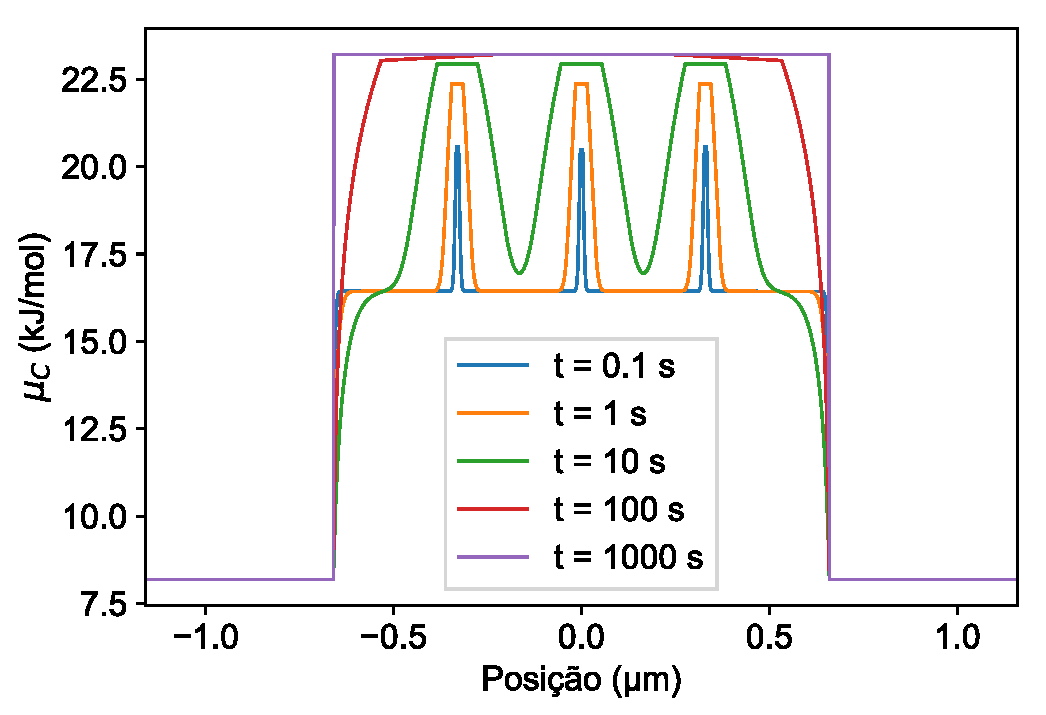
\includegraphics[width=.8\textwidth]{img/cpartition/muprofiles/coupled_FoFo_375_CCEortho.pdf}
  \caption{Perfis de potencial químico de carbono $\mu_C$ correspondentes aos perfis de carbono mostrados na Figura \ref{fig:muprofiles_coupled_CCEortho}, isto é, para o caso em que são considerados a reação bainítica e a precipitação de ortocementita na martensita.}
  \label{fig:muprofiles_coupled_CCEortho}
\end{figure}

A Figura \ref{fig:cprofiles_coupled_CCEpara} mostra os perfis de carbono para quando a precipitação de paracementita na martensita é considerada. De forma semelhante ao que acontece nos casos em que não há bainita, quando há a precipitação de paracementita, a cinética de redistribuição de carbono se assemelha muito à situação em que não há qualquer precipitação de carbonetos. Para tempos curtos ocorre rápida partição da martensita para a austenita, acompanhada da dissolução total dos carbonetos, e para tempos longos as placas de ferrita bainítica próximas à martensita dissolvem parcialmente.

\begin{figure}
  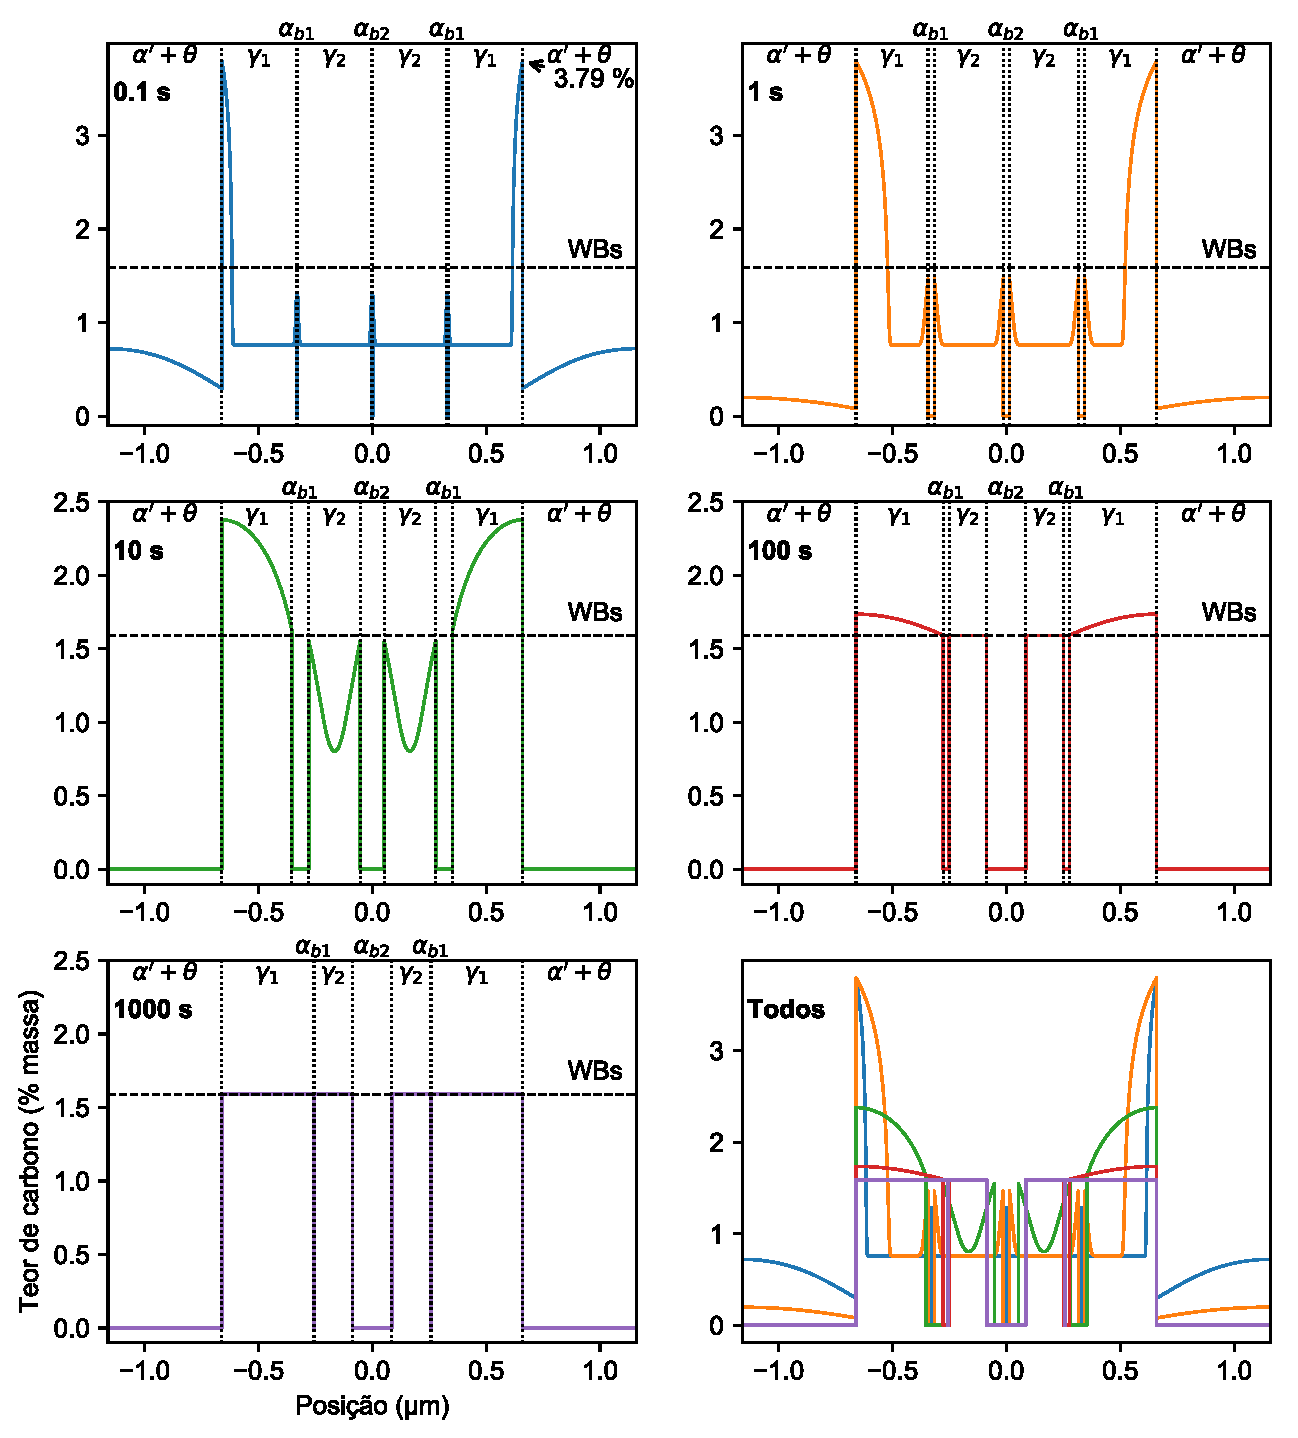
\includegraphics[width=.9\textwidth]{img/cpartition/cprofiles/coupled_FoFo_375_CCEpara_sep.pdf}
  \caption{Perfis de carbono calculados para o caso em que é assumida a precipitação de paracementita na martensita e ocorre reação bainítica na austenita.}
  \label{fig:cprofiles_coupled_CCEpara}
\end{figure}

Como discutido anteriormente, isto está diretamente relacionado ao fato de que a composição interfacial $c^\gamma_{int}$ resultante assume um valor alto, elevando o coeficiente de difusão do carbono na austenita na interface. Tanto neste caso, quanto na situação sem carbonetos, todo o carbono é particionado da martensita para a austenita antes de que os perfis de difusão de carbono na austenita sofram \enfase{soft impingement}. Isto é, quando a partição de carbono já está praticamente finalizada, o perfil de carbono decorrente do crescimento da ferrita bainítica ainda não se interage com o perfil de carbono particionado da martensita. Este fenômeno pode ser claramente observado a $t = \SI{1}{s}$ nas simulações mencionadas. 

Um terceiro cenário simulado é mostrado na Figura \ref{fig:cprofiles_coupled_mu23e3}. Neste caso a energia livre dos carbonetos foi deliberadamente escolhida para representar uma situação intermediária em que a composição interfacial na austenita determinada pelo modelo ERC$\theta$ coincide com a composição WBs. Nesta situação, o potencial químico local de carbono é $\mu_C = \SI{23.207}{kJ/mol}$. Uma vez que neste caso os limites termodinâmicos para crescimento de $\alpha_b$ e partição de carbono são ambos a composiação WBs, ao final da simulação os perfis de carbono em todos os blocos de austenita estabelecem um patamar. O carbono em $\alpha' + \theta$ descresce até também atingir um patamar a aproximadamente 0,58\%, correspondente a $\approx$~8,9\%~vol. de carbonetos na martensita. Nesta situação de equilíbrio, portanto, martensita, carbonetos, austenita e ferrita bainítica estabelecem o equilíbrio entre si.

\begin{figure}
  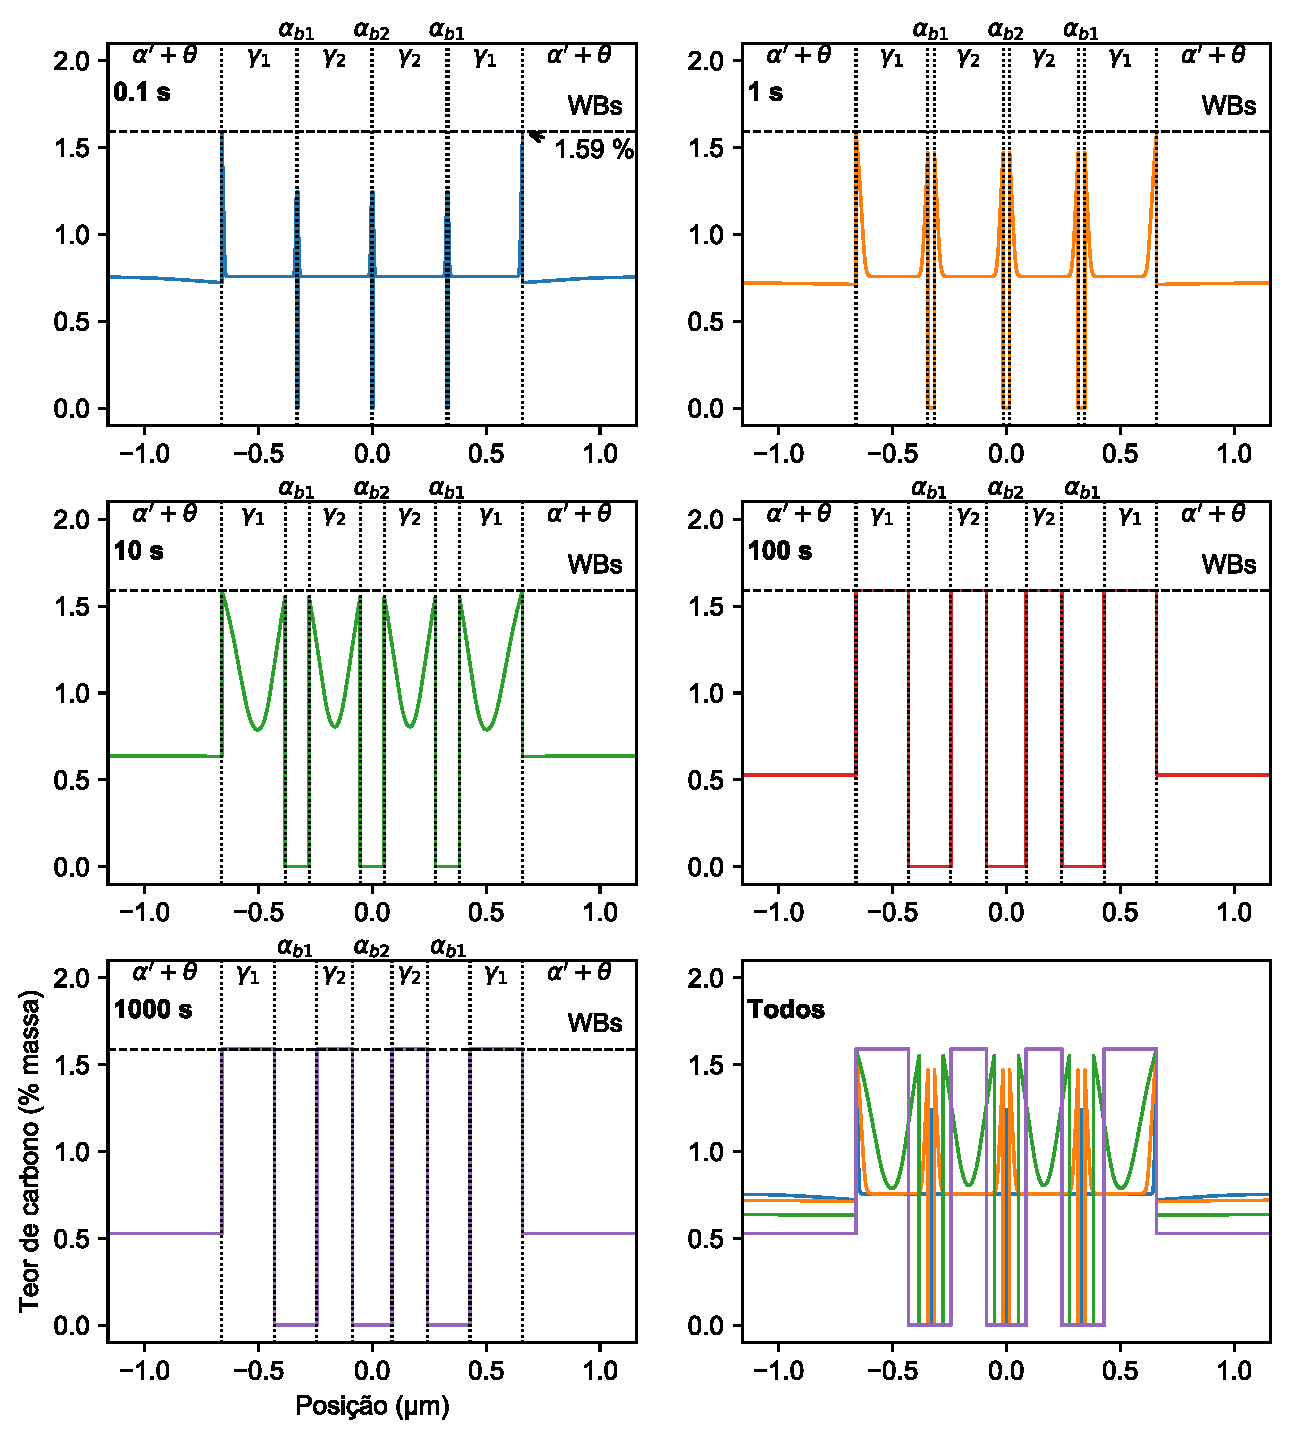
\includegraphics[width=.9\textwidth]{img/cpartition/cprofiles/coupled_FoFo_375_mu23e3_sep.pdf}
  \caption{Perfis de carbono calculados para o caso em que é assumida a ocorrência de reação bainítica e considera-se a precipitação na martensita de um carboneto com o potencial químico de carbono correspondente a $\mu_C = \SI{23e3}{J/mol}$. Nesta condição, a composição da austenita na interface $\alpha' + \theta/\gamma$ equivale à composição WBs.}
  \label{fig:cprofiles_coupled_mu23e3}
\end{figure}

Na Figura \ref{fig:coupled_cavg} a cinética da partição do carbono da martensita ou pseudofase $\alpha' + \theta$ para a austenita é avaliada em termos da evolução da composição média de $\alpha' + \theta$ ($\overline{c^{\alpha' + \theta}}$) para tempos crescentes de partição. Na figura são apresentados não somente os resultados dos perfis de carbono, mas todas as condições simuladas assumindo formação de bainita, sumarizadas na Tabela \ref{tab:cpartition_bainite_CCEtheta}.

\begin{figure}
  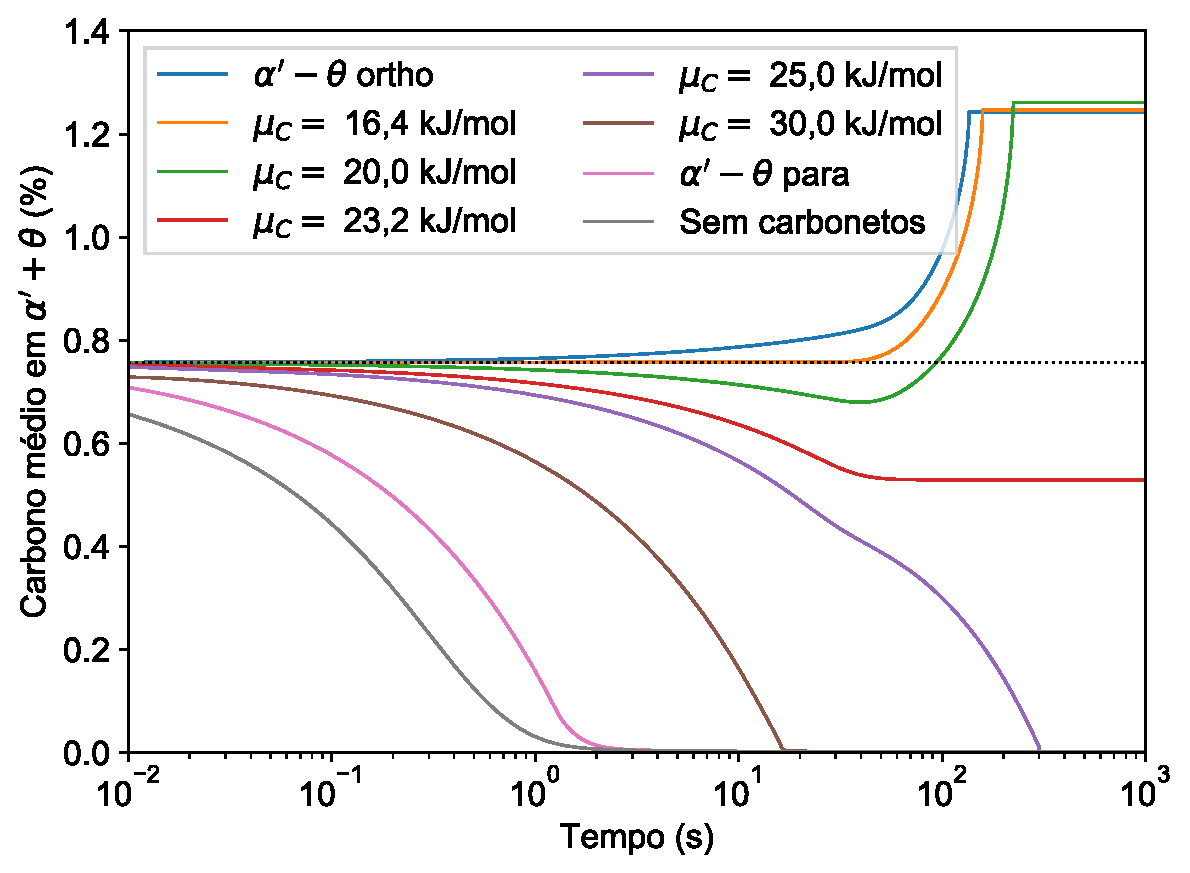
\includegraphics[height=.6\textwidth]{img/cpartition/coupled_cavg.pdf}
  \caption{Evolução do teor de carbono médio na pseudofase $\alpha' + \theta$ ($\overline{c^{\alpha' + \theta}}$) com o tempo de partição calculada para os cenários em que é considerada a reação bainítica e precipitação de carbonetos com diferentes energias livres.}
  \label{fig:coupled_cavg}
\end{figure}

As condições de simulação e os diferentes comportamentos cinéticos observados na Figura \ref{fig:coupled_cavg} podem ser separados nas seguintes diferentes categorias, de acordo com o valor de $c^\gamma_{int}$ relativo às composições inicial e WBs:

\begin{itemize}
  \item $c^\gamma_{int} \leq c_0 < WBs$: A composição interfacial na austenita é inferior ao teor inicial de carbono;
  % Acontece na situação de precipitação de ortocementita;
  % \item $c_0 = c^\gamma_{int} < WBs$: A composição interfacial é igual à composição inicial.
  \item $c_0 < c^\gamma_{int} \leq WBs$: A composição interfacial é maior do que a composição inicial, mas é inferior à composição WBs;
  % \item $c_0 < c^\gamma_{int} = WBs$: A composição interfacial é igual à composição WBs. Acontece somente se $\mu_C = \SI{23.207}{kJ/mol}$;
  \item $c_0 < WBs < c^\gamma_{int}$: A composição interfacial é superior à composição WBs.
  % É o caso das condições $\mu_C = \SI{30}{kJ/mol}$ e precipitação de paracementita.
\end{itemize}

Quando $c^\gamma_{int}$ é inferior a $c_0$ ($\mu_C < \SI{16.434}{kJ/mol}$), como acontece quando há precipitação de ortocementita, a configuração do sistema favorece a difusão de carbono da austenita para a mistura de martensita + cementita. Tal situação pode ocorrer em qualquer cenário em que os carbonetos precipitados são suficientemente estáveis. Para tempos longos o carbono rejeitado para a austenita pelo crescimento da ferrita bainítica passa a interagir com o carbono proveniente de $\alpha' + \theta$, aumentando ainda mais o gradiente de carbono à frente da interface $(\alpha' + \theta)/\gamma$. Isso faz com que o enriquecimento em carbono de $\alpha' + \theta$ --- traduzido na forma do aumento da fração de carbonetos --- acelere. Na Figura \ref{fig:all_cavg}, em que é mostrada a sobreposição das curvas de $\overline{c^{\alpha' + \theta}}$ calculadas com e sem a presença de carbonetos, esta aceleração é claramente visível pelo desvio da curva sólida, correspondente à condição com formação de bainita, da curva tracejada, sem formação de bainita.

\begin{figure}
  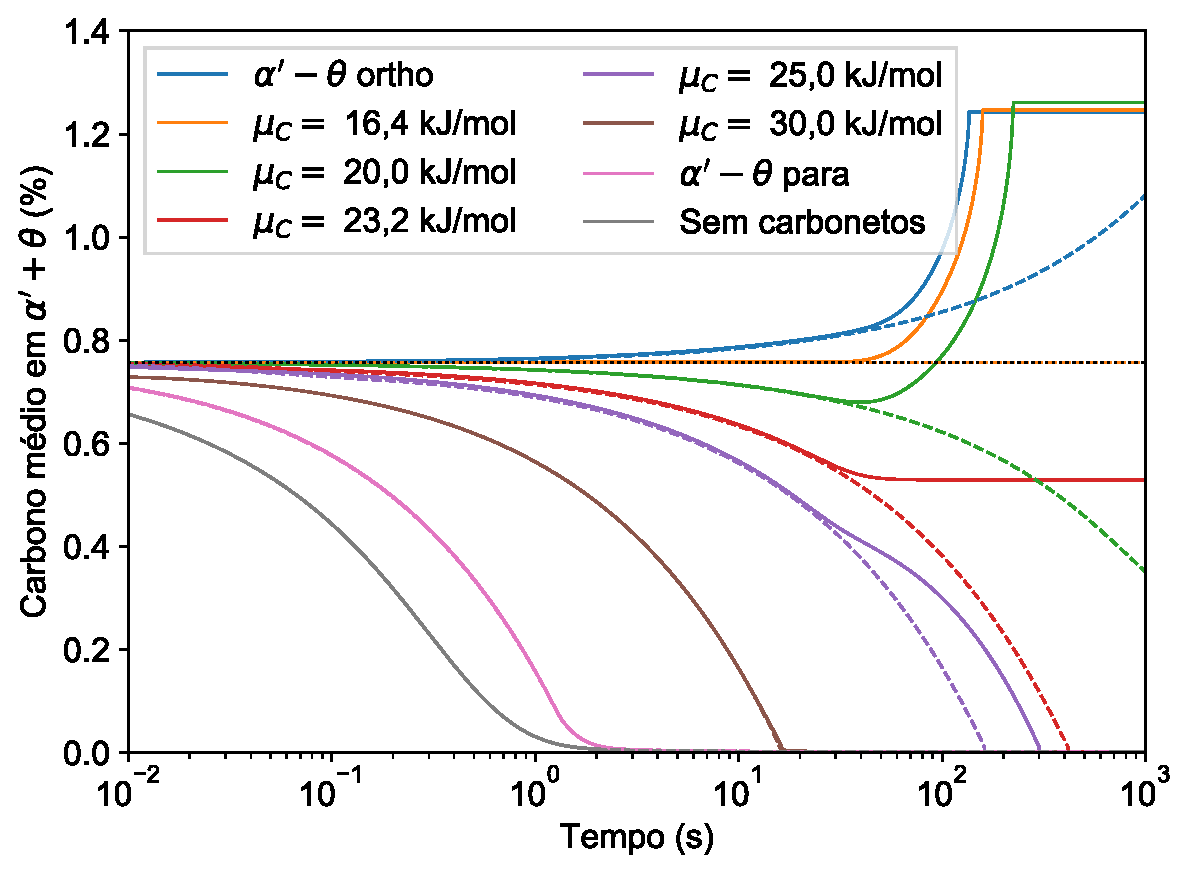
\includegraphics[height=.6\textwidth]{img/cpartition/all_cavg.pdf}
  \caption{Evolução de $\overline{c^{\alpha' + \theta}}$ para todos os casos simulados em que é assumida a precipitação de carbonetos. Linhas sólidas representam os cenários em que também é assumida a reação bainítica (equivalente à Figura \ref{fig:coupled_cavg}); linhas tracejadas correspondem aos cenários sem bainita (Figura \ref{fig:nobainite_cavg}).}
  \label{fig:all_cavg}
\end{figure}

Por outro lado, como mostrado na seção \ref{sec:cpartition_sem_bainita}, para qualquer outra condição em que $c^\gamma_{int}$ é maior do que $c_0$, a partição de carbono da martensita para a austenita é termodinamicamente possível. Isso leva inicialmente à diminuição de $\overline{c^{\alpha' + \theta}}$. Entretanto, a interação (\enfase{soft impingement}) na austenita do carbono proveniente de $\alpha' + \theta$ e $\alpha_b$ determina a evolução de $\overline{c^{\alpha' + \theta}}$ para tempos longos. Nas simulações sem bainita o \enfase{soft impingement} tem o efeito de atenuar os gradientes de carbono até que um patamar de carbono é atingido na austenita. Nos casos que levam em conta a ferrita bainítica, como diferentes composições interfaciais são definidas nas interfaces $(\alpha' + \theta)/\gamma$ e $\alpha_b/\gamma$, tal atenuação ocorre apenas para condições muito específicas.

Caso $c^\gamma_{int}$ seja maior do que $c_0$, mas menor do que WBs, como para $\mu_C = \SI{20}{kJ/mol}$, o gradiente de carbono à frente da interface martensita/austenita produzido pela interação dos perfis de carbono faz com que a partição mude de sentido e passe a enriquecer a $\alpha' + \theta$ em carbono. Para $\mu_C = \SI{20}{kJ/mol}$ isto acontece a aproximadamente 40~s. No entanto, note-se que $\overline{c^{\alpha' + \theta}}$ vem a se tornar maior do que a composição inicial apenas após cerca de 100~s. Dessa forma, para tratamentos curtos, inferiores a 100~s, o balanço de carbono é favorável ao enriquecimento da austenita pela partição de carbono da martensita. Caso $c^\gamma_{int}$ seja exatamente igual a WBs ($\mu_C = \SI{23.207}{kJ/mol}$), tem-se a condição específica em que um patamar de carbono é obtido na austenita, tal qual mostrado nos perfis de carbono na Figura \ref{fig:cprofiles_coupled_mu23e3}. Consequentemente, a curva de $\overline{c^{\alpha' + \theta}}$ também estabelece um patamar a $\approx$~0,58\%, equivalente a $\approx$~8,9\%~vol. de $\theta$.

Para qualquer valor de $c^\gamma_{int}$ superior a WBs, tem-se uma situação semelhante ao caso em que não há precipitação de carbonetos. Embora a presença de carbonetos claramente diminua a cinética de partição de carbono de $\alpha' + \theta$ para $\gamma$, termodinamicamente não há impedimento para que todo carbono seja particionado. Caso a diferença entre $c^\gamma_{int}$ e WBs seja pequena, é possível que o \enfase{soft impingement} ocorra antes de que todo o carbono seja particionado de $\alpha' + \theta$ para $\gamma$, de modo que a cinética de partição é atrasada em relação ao caso em que não há bainita. Na Figura \ref{fig:all_cavg} é possível ver que isto acontece para a condição em que $\mu_C = \SI{25}{kJ/mol}$. Para maiores valores de $\mu_C$, observa-se que a ocorrência da reação bainítica não exerce nenhuma influência na cinética de partição de carbono. Isso é explicado pelo fato de a partição de carbono ser completada antes de que o \enfase{soft impingement} na austenita ocorra.

O modelo prevê que a partição de carbono para a austenita depende de qual fase a austenita faz fronteira. O teor de carbono de blocos de austenita presos entre placas de ferrita bainítica irão atingir a composição WBs. Blocos de austenita entre a martensita e a bainita atingirão composições entre as composições determinadas pelos modelos ERC$\theta$ e WBs, pelo menos para tempos curtos, enquanto a austenita não for completamente consumida. Finalmente, blocos de austenita entre placas de martensita terão o carbono limitado pela composição ERC$\theta$. A última situação é menos frequente, uma vez que interfaces $\alpha'/\gamma$ são parcialmente eliminadas por nucleação simpática de placas de bainita. As outras duas situações ocorrem mais frequentemente. Uma vez que placas de bainita são mais finas do que placas de martensita na liga simulada de alto carbono, é esperado que o primeiro caso seja dominante. Em particular, austenita retida em regiões de contorno de célula, que apresentam fração próxima de zero de martensita, terá sua composição definida pela composição WBs.
Abaixando a temperatura de têmpera tem o efeito de criar mais interfaces $\alpha'/\gamma$, abaixando assim a composição da austenita após a etapa de partição para valores mais próximos daqueles estimados pelo modelo ERC$\theta$.

% It should be emphasized that in the studied alloy bainite reaction controls the carbon enrichment of austenite because of its fast reaction kinetics. Recent Q\&P steels have been designed with high amounts of alloying elements (such as Mn and Ni) in order to improve the hardenability and avoid austenite decomposition during partitioning step \cite{Santofimia2011,Goune2013,Toji2015}. However, increased alloying addition has the side effect of enlarge the microsegregation effects discussed in this work, particularly for cast products that are not submitted to a previous homogenization treatment.

% The experimental evidence for carbon partitioning for short times at 375~°C and persistence of undissolved transition carbides for longer times are indication that the experimental results are compatible with the scenario where $c_0 < c^\gamma_{int} < WBs$.
% % $16.434 < \mu_C < 23.207~kJ/mol$
% A similar situation is expected at 300~°C because transition carbides are also formed in this condition. At 450~°C transition carbides are probably present for short times, allowing carbon partitioning from $\alpha' + \theta$ to $\gamma$. For longer times cementite is formed and the austenite interfacial composition decreases, eventually dropping to values below $c_0$, favoring the dissolution of austenite by bainite reaction. Simultaneously, cementite precipitation occurs in bainite, which also contributes to austenite decomposition.


% TABELA COMPARANDO MODELO E REGRA DAS ALAVANCAS WBS
% 
% 



